% !TEX root = smc_bandits.tex

We here apply the proposed SMC-based Bayesian policies as in Algorithm~\ref{alg:sir-mab}
to the original settings where Thompson sampling and Bayes-UCB were derived,
\ie for stationary bandits with Bernoulli and contextual, linear Gaussian reward functions~\cite{ip-Kaufmann2012,ip-Garivier2011a,ic-Korda2013,ip-Agrawal2013a}.

Empirical results for these bandits is provided in Section~\ref{assec:static_bandits_experiments_analytical},
while the stationary logistic bandit case is evaluated in Section~\ref{assec:static_bandits_experiments_logistic},
where we also evaluate the impact of sample size $M$ in the SMC-based bandit algorithms.

\subsection{SMC-based policies for stationary bandits}
\label{assec:static_bandits_smc}
In stationary bandits, 
there are no time-varying parameters, \ie $\theta_t=\theta, \ \forall t$.
For these cases, SIR-based parameter propagation becomes troublesome \cite{b-Liu2001}.
To mitigate such issues, several alternatives have been proposed in the SMC community:
\eg artificial parameter evolution \cite{j-Gordon1993},
kernel smoothing \cite{b-Liu2001}, and density assisted techniques \cite{ip-Djuric2004}.

We implement density assisted SMC,
rather than kernel based particle filters as in~\cite{j-Cherkassky2013},
where one approximates the posterior of the unknown parameters with a density of choice.
%
Density assisted importance sampling is a well studied SMC approach
that extends random-walking and kernel-based alternatives~\cite{j-Gordon1993, ib-Liu2001, ip-Djuric2004},
with its asymptotic correctness guaranteed for the static parameter case.
We acknowledge that any of the SMC techniques that further mitigate
the challenges of estimating constant parameters
(\eg parameter smoothing~\cite{j-Carvalho2010,j-Olsson2006,j-Olsson2014}
or nested SMC methods~\cite{j-Chopin2011,j-Crisan2013})
can only improve the accuracy of the implemented SMC-based policies. 

More precisely,
we approximate the posterior of the unknown parameters,
given the current state of knowledge,
with a Gaussian distribution
\begin{equation}
p(\theta_a|\HH_{1:t}) \approx \N{\theta_a|\hat{\theta}_{t,a}, \hat{\Sigma}_{\theta_{t,a}}},
\end{equation}
based on the updated random measure.
Namely, the sufficient statistics of the distribution 
are estimated based on samples and weights of the SMC random measure $p_M(\theta_{t,a})=\sum_{m=1}^M w_{t}^{(m)} \delta\left(\theta_{t,a}-\theta_{t,a}^{(m)}\right)$,
available at each bandit interaction; \ie
\begin{equation}
\begin{split}
\hat{\theta}_{t,a} &= \sum_{i=1}^{M} w_{t,a}^{(m)} \theta^{(m)}_{t,a} \;,  \\
\hat{\Sigma}_{\theta_{t,a}} &= \sum_{i=1}^{M} w_{t,a}^{(m)}(\theta^{(m)}_{t,a} - \hat{\theta}_{t,a})(\theta^{(m)}_{t,a} - \hat{\theta}_{t,a})^\top \;.
\end{split}
\label{eq:proposedMethod_unknownAB_DA_estSuffStatistics}
\end{equation}
Hence, when addressing static bandits,
we slightly modify Algorithm~\ref{alg:sir-mab},
and propagate parameters in Steps 5 and 9-b,
by drawing from
\begin{equation}
p(\theta_{t+1,a}|\theta_{t,a})=p(\theta_{t,a}|\HH_{1:t}) \approx \N{\theta_{t,a}|\hat{\theta}_{t,a}, \hat{\Sigma}_{\theta_{t,a}}} \;.
\end{equation}

\subsection{Experiments with SMC-based Bayesian policies for Bernoulli and Gaussian stationary bandits}
\label{assec:static_bandits_experiments_analytical}

We provide results for stationary bandits with 2 and 5 arms,
for Bernoulli rewards in Sections~\ref{asssec:static_bandits_bernoulli_2} \& \ref{asssec:static_bandits_bernoulli_5},
and contextual-Gaussian rewards in Sections~\ref{asssec:static_bandits_linearGaussian_2} \& \ref{asssec:static_bandits_linearGaussian_5}, respectively.

Provided empirical evidence showcases
how the proposed SMC-based Bayesian policies perform satisfactorily in both stationary bandit settings.
The more realistic assumption of unknown reward variance $\sigma^2$ for the contextual, linear Gaussian case is also evaluated,
where SMC-based policies are shown to be equally competitive.

We observe that, as the posterior random measure $p_M(\theta_{t,a})$ becomes more accurate, \eg for $M\geq 500$,
SMC-based TS and UCB perform similarly to their counterpart benchmark policies that make use of analytical posteriors.

We note a increased performance uncertainty due to the SMC posterior random measure,
which is empirically reduced by increasing the number $M$ of Monte Carlo samples:
we illustrate the impact of sample size $M$ in the provided figures.

In general, $M=1000$ samples suffice in our static bandit experiments for accurate estimation of parameter posteriors.
Advanced and dynamic determination of SMC sample size is an active research area, out of the scope of this paper.

%\clearpage
% !TEX root = smc_bandits.tex

\subsubsection{Bernoulli bandits, A=2}
\label{asssec:static_bandits_bernoulli_2}

We present below cumulative regret results for different parameterizations of 2-armed Bernoulli bandits.

% (0.1, 0.2)
\begin{figure}[!h]
	\centering
	\begin{subfigure}[b]{\textwidth}
		\centering
		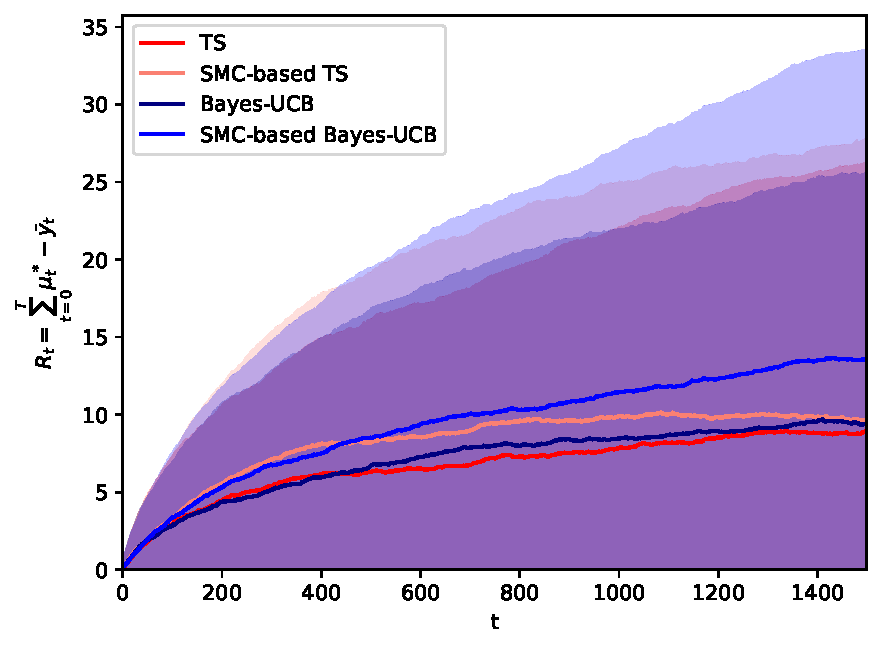
\includegraphics[width=0.75\textwidth]{./fods_figs/static/bernoulli/A2/theta0.1_0.2_M1000_cumulative_regret}
		\caption{Analytical and SMC-based ($M=1000$) TS and Bayes-UCB.}
	\end{subfigure}
	
	\begin{subfigure}[b]{0.46\textwidth}
		\centering
		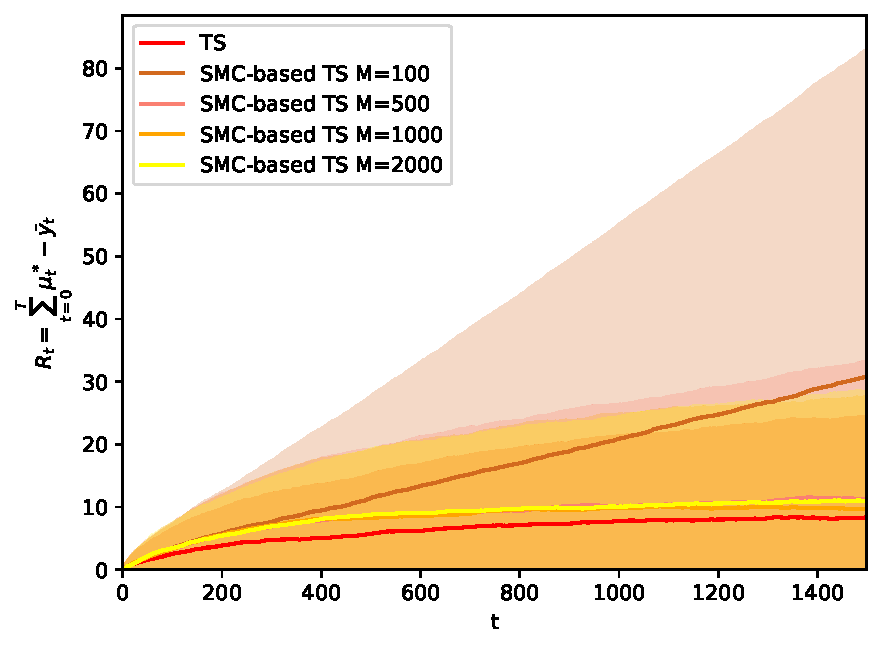
\includegraphics[width=\textwidth]{./fods_figs/static/bernoulli/A2/theta0.1_0.2_allM_cumulative_regret_ts}
		\caption{SMC-based TS: impact of $M$.}
	\end{subfigure}
	\begin{subfigure}[b]{0.46\textwidth}
		\centering
		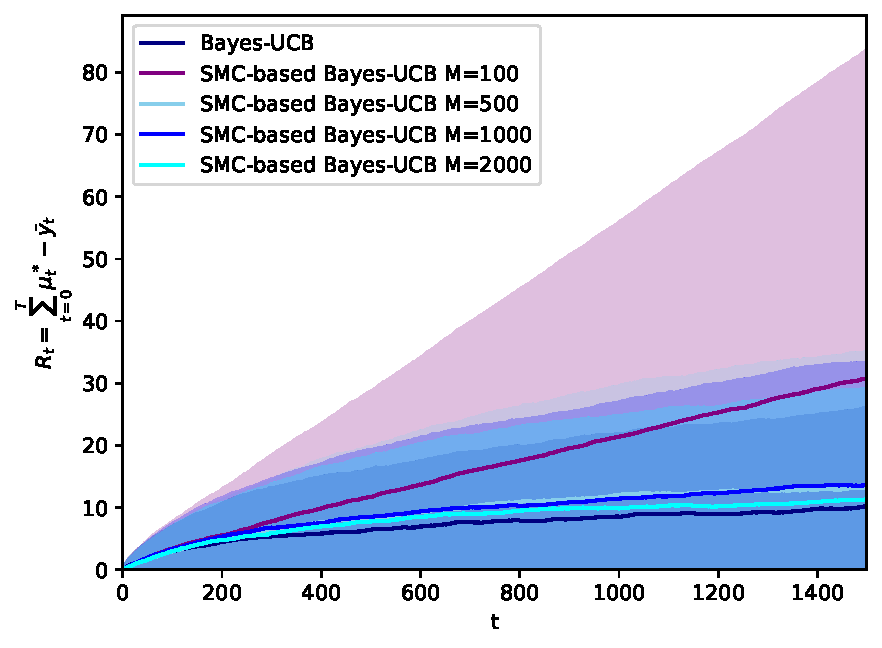
\includegraphics[width=\textwidth]{./fods_figs/static/bernoulli/A2/theta0.1_0.2_allM_cumulative_regret_bucb}
		\caption{SMC-based Bayes-UCB: impact of $M$}
	\end{subfigure}
	
	\caption{Mean cumulative regret (standard deviation shown as the shaded region) of Bayesian policies in a stationary two-armed Bernoulli bandit, with $\theta_0=0.1, \ \theta_1=0.2$.}
\end{figure}

% (0.1, 0.3)
\begin{figure}[!h]
	\centering
	\begin{subfigure}[b]{\textwidth}
		\centering
		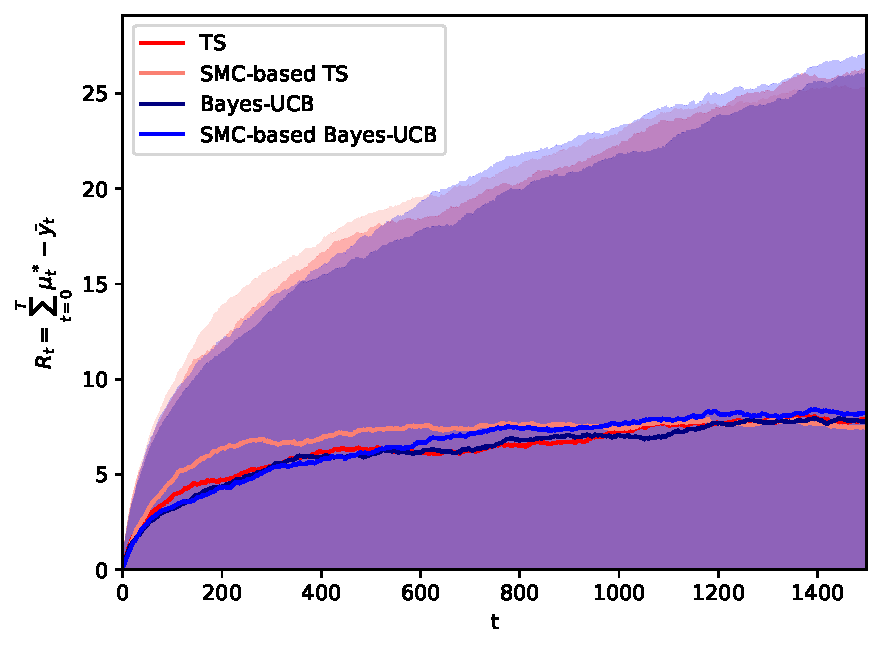
\includegraphics[width=0.75\textwidth]{./fods_figs/static/bernoulli/A2/theta0.1_0.3_M1000_cumulative_regret}
		\caption{Analytical and SMC-based ($M=1000$) TS and Bayes-UCB.}
	\end{subfigure}
	
	\begin{subfigure}[b]{0.46\textwidth}
		\centering
		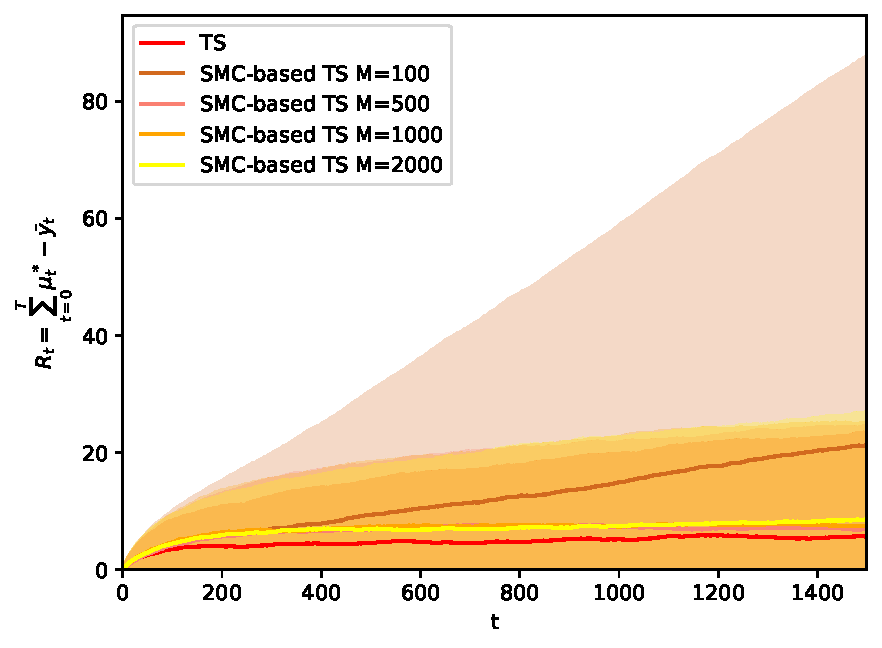
\includegraphics[width=\textwidth]{./fods_figs/static/bernoulli/A2/theta0.1_0.3_allM_cumulative_regret_ts}
		\caption{SMC-based TS: impact of $M$.}
	\end{subfigure}
	\begin{subfigure}[b]{0.46\textwidth}
		\centering
		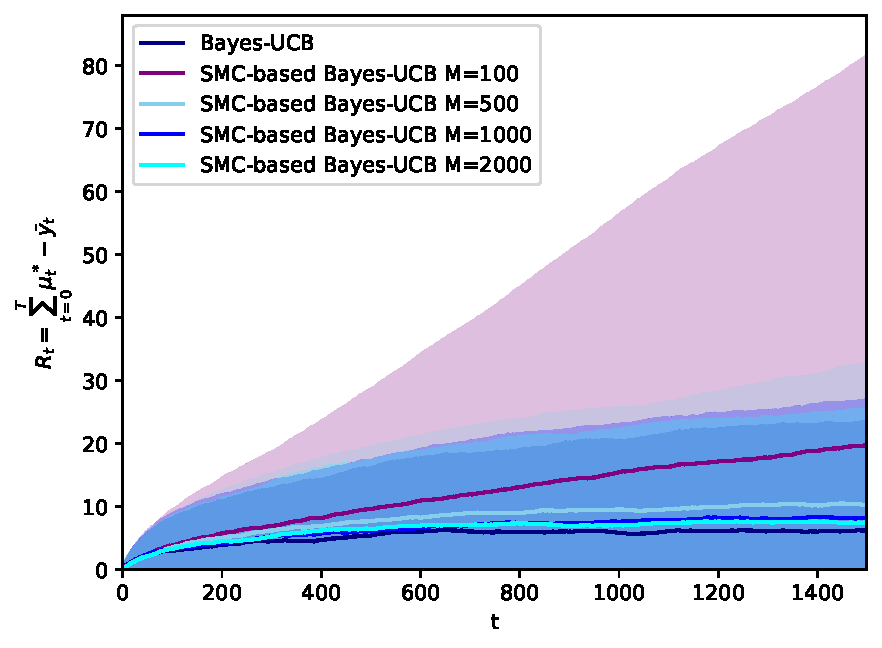
\includegraphics[width=\textwidth]{./fods_figs/static/bernoulli/A2/theta0.1_0.3_allM_cumulative_regret_bucb}
		\caption{SMC-based Bayes-UCB: impact of $M$}
	\end{subfigure}
	
	\caption{Mean cumulative regret (standard deviation shown as the shaded region) of Bayesian policies in a stationary two-armed Bernoulli bandit, with $\theta_0=0.1, \ \theta_1=0.3$.}
\end{figure}

% (0.5, 0.6)
\begin{figure}[!h]
	\centering
	\begin{subfigure}[b]{\textwidth}
		\centering
		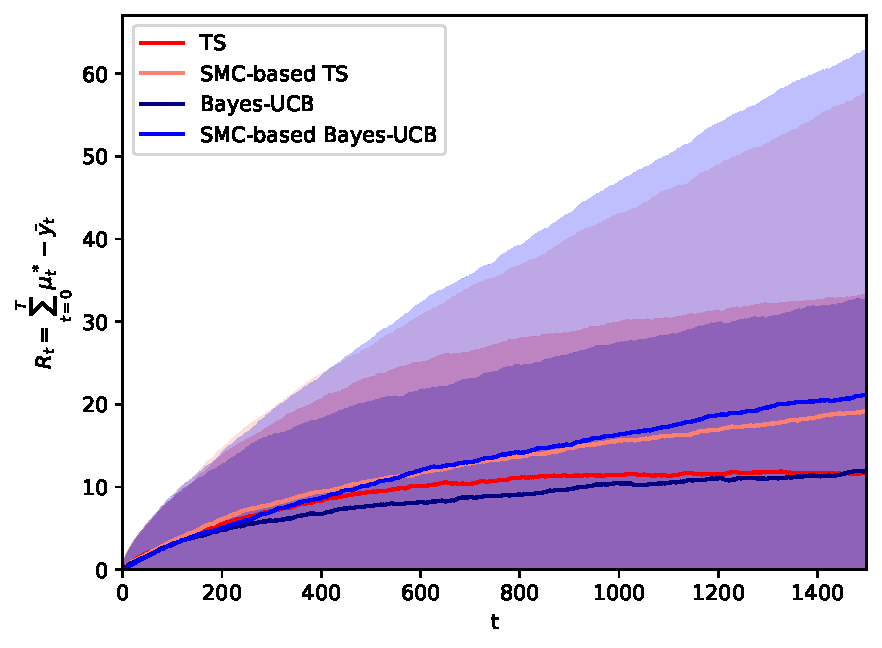
\includegraphics[width=0.75\textwidth]{./fods_figs/static/bernoulli/A2/theta0.5_0.6_M1000_cumulative_regret}
		\caption{Analytical and SMC-based ($M=1000$) TS and Bayes-UCB.}
	\end{subfigure}
	
	\begin{subfigure}[b]{0.46\textwidth}
		\centering
		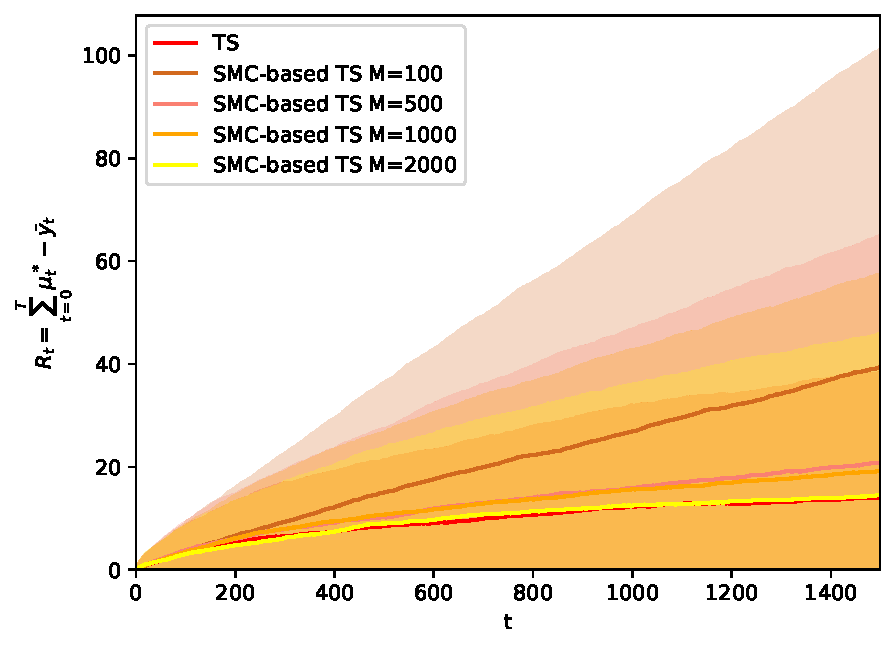
\includegraphics[width=\textwidth]{./fods_figs/static/bernoulli/A2/theta0.5_0.6_allM_cumulative_regret_ts}
		\caption{SMC-based TS: impact of $M$.}
	\end{subfigure}
	\begin{subfigure}[b]{0.46\textwidth}
		\centering
		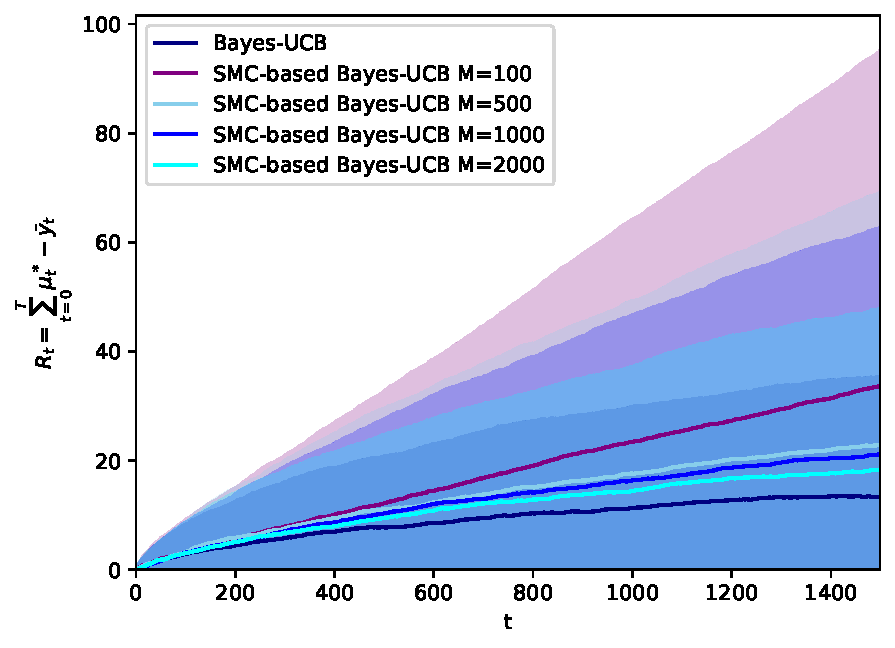
\includegraphics[width=\textwidth]{./fods_figs/static/bernoulli/A2/theta0.5_0.6_allM_cumulative_regret_bucb}
		\caption{SMC-based Bayes-UCB: impact of $M$}
	\end{subfigure}
	
	\caption{Mean cumulative regret (standard deviation shown as the shaded region) of Bayesian policies in a stationary two-armed Bernoulli bandit, with $\theta_0=0.5, \ \theta_1=0.6$.}
\end{figure}

% (0.5, 0.7)
\begin{figure}[!h]
	\centering
	\begin{subfigure}[b]{\textwidth}
		\centering
		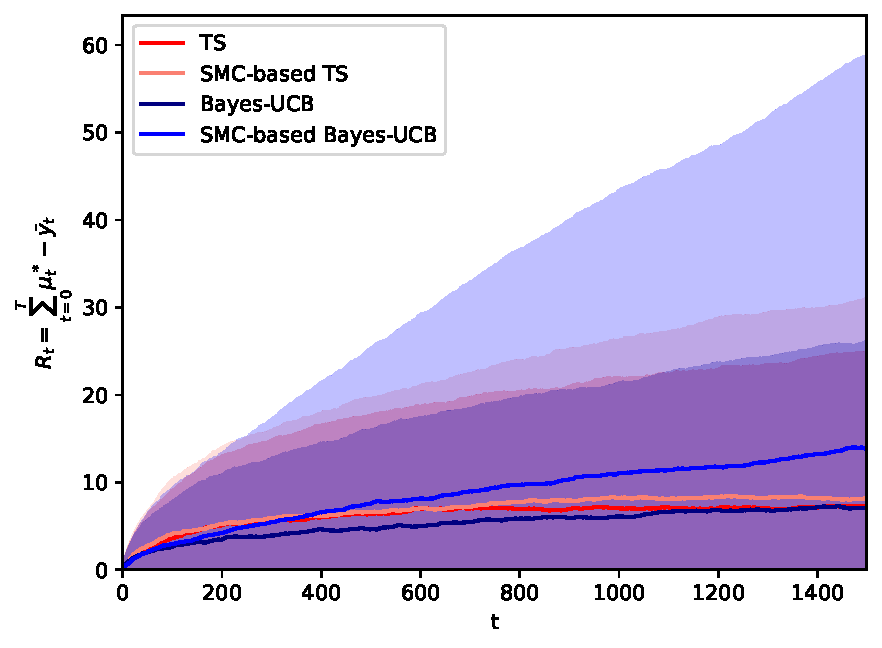
\includegraphics[width=0.75\textwidth]{./fods_figs/static/bernoulli/A2/theta0.5_0.7_M1000_cumulative_regret}
		\caption{Analytical and SMC-based ($M=1000$) TS and Bayes-UCB.}
	\end{subfigure}
	
	\begin{subfigure}[b]{0.46\textwidth}
		\centering
		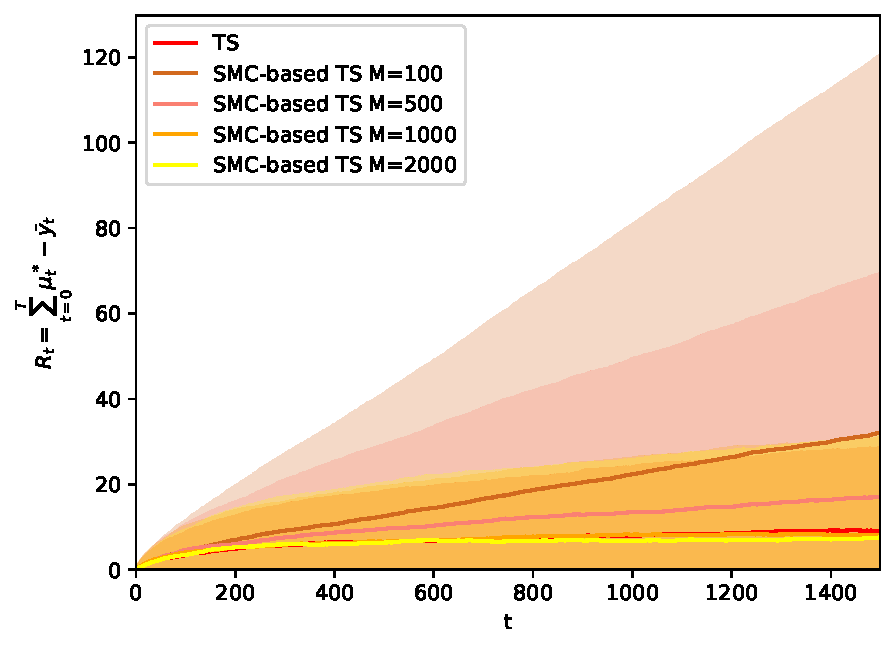
\includegraphics[width=\textwidth]{./fods_figs/static/bernoulli/A2/theta0.5_0.7_allM_cumulative_regret_ts}
		\caption{SMC-based TS: impact of $M$.}
	\end{subfigure}
	\begin{subfigure}[b]{0.46\textwidth}
		\centering
		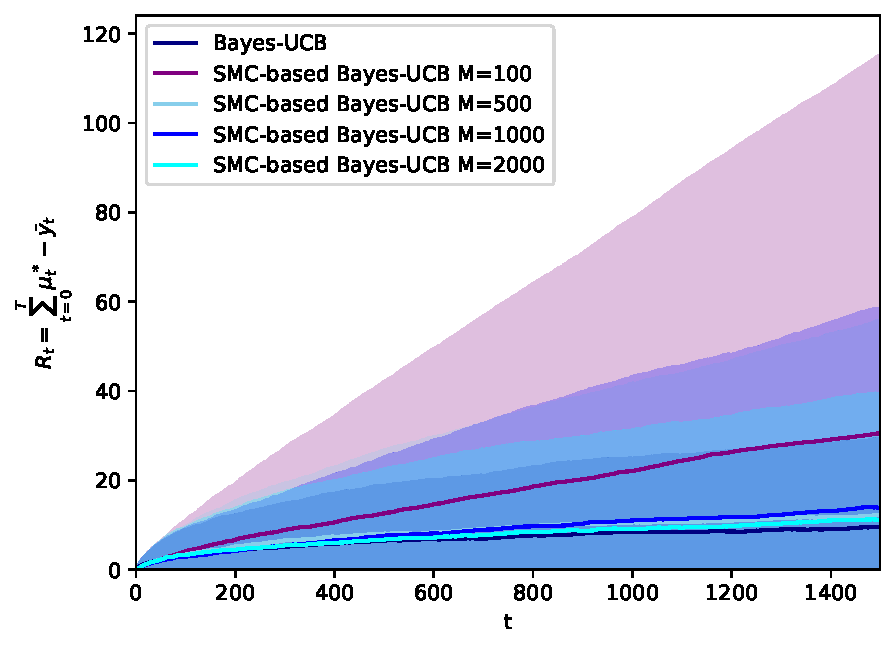
\includegraphics[width=\textwidth]{./fods_figs/static/bernoulli/A2/theta0.5_0.7_allM_cumulative_regret_bucb}
		\caption{SMC-based Bayes-UCB: impact of $M$}
	\end{subfigure}
	
	\caption{Mean cumulative regret (standard deviation shown as the shaded region) of Bayesian policies in a stationary two-armed Bernoulli bandit, with $\theta_0=0.5, \ \theta_1=0.7$.}
\end{figure}

% (0.7, 0.9)
\begin{figure}[!h]
	\centering
	\begin{subfigure}[b]{\textwidth}
		\centering
		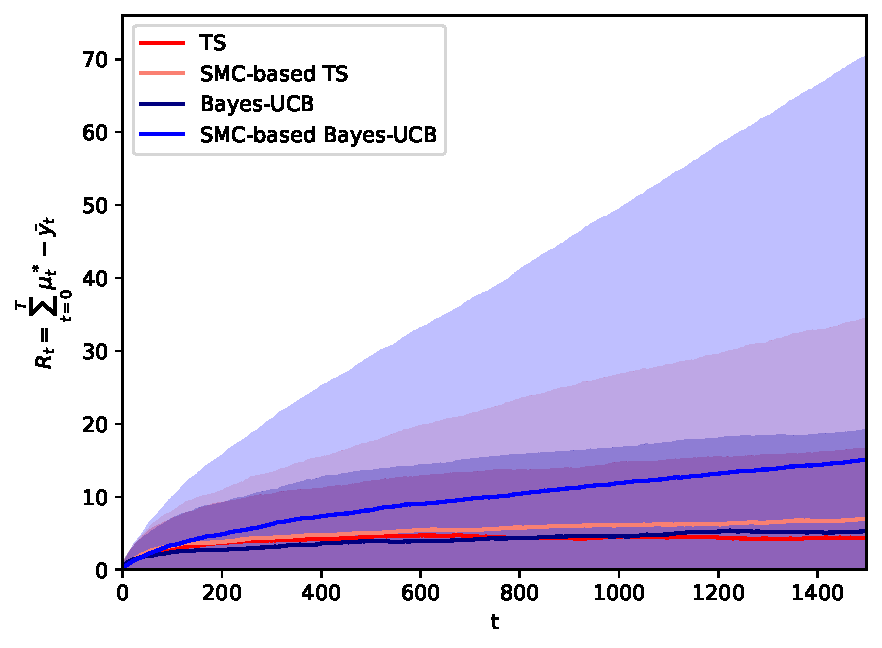
\includegraphics[width=0.75\textwidth]{./fods_figs/static/bernoulli/A2/theta0.7_0.9_M1000_cumulative_regret}
		\caption{Analytical and SMC-based ($M=1000$) TS and Bayes-UCB.}
	\end{subfigure}
	
	\begin{subfigure}[b]{0.46\textwidth}
		\centering
		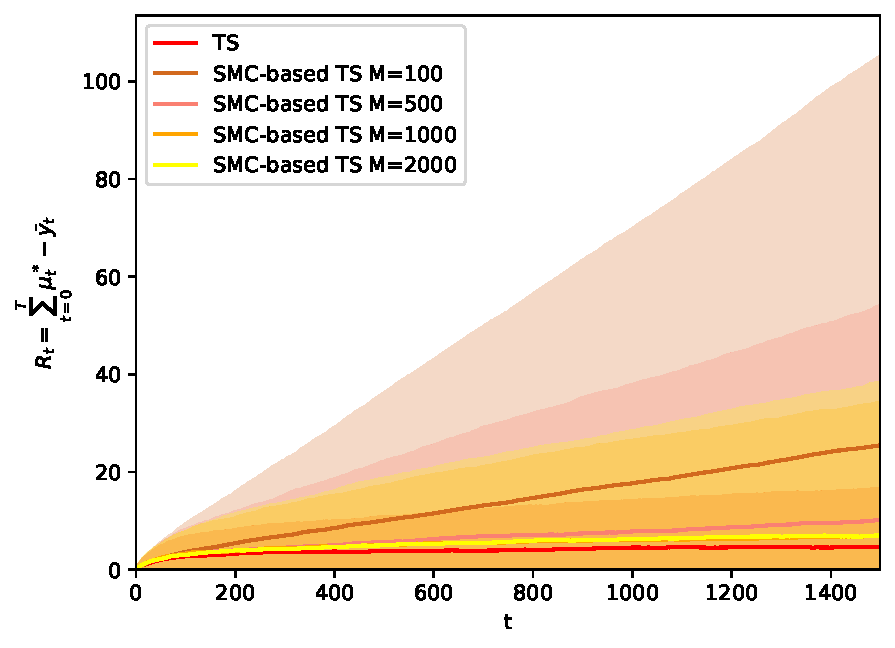
\includegraphics[width=\textwidth]{./fods_figs/static/bernoulli/A2/theta0.7_0.9_allM_cumulative_regret_ts}
		\caption{SMC-based TS: impact of $M$.}
	\end{subfigure}
	\begin{subfigure}[b]{0.46\textwidth}
		\centering
		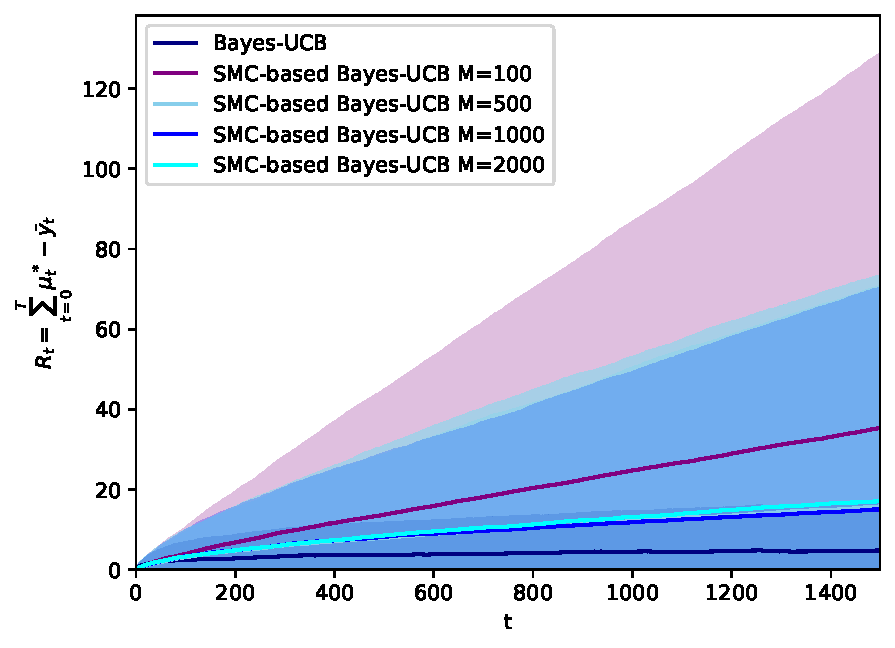
\includegraphics[width=\textwidth]{./fods_figs/static/bernoulli/A2/theta0.7_0.9_allM_cumulative_regret_bucb}
		\caption{SMC-based Bayes-UCB: impact of $M$}
	\end{subfigure}
	
	\caption{Mean cumulative regret (standard deviation shown as the shaded region) of Bayesian policies in a stationary two-armed Bernoulli bandit, with $\theta_0=0.7, \ \theta_1=0.9$.}
\end{figure}

% (0.8, 0.9)
\begin{figure}[!h]
	\centering
	\begin{subfigure}[b]{\textwidth}
		\centering
		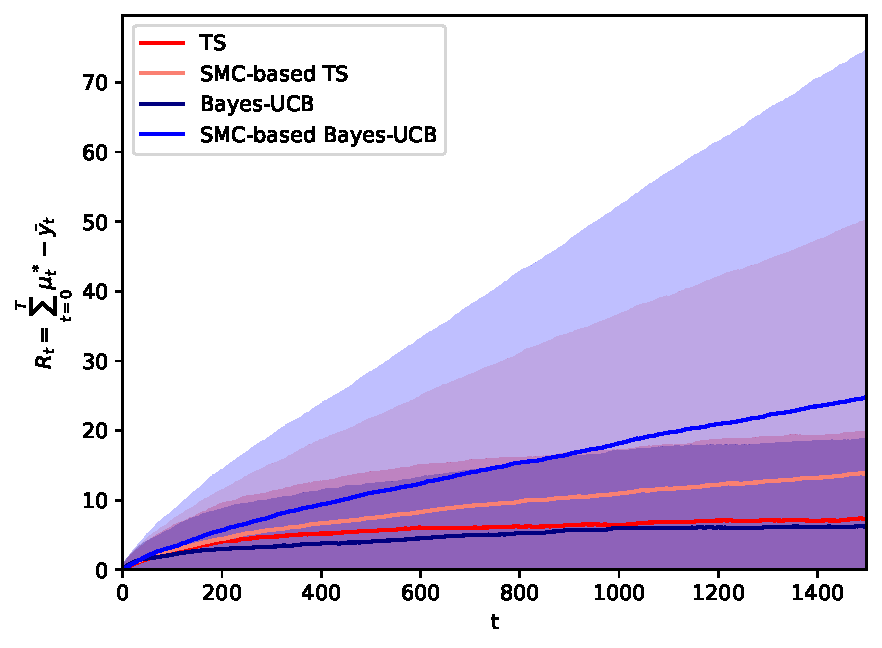
\includegraphics[width=0.75\textwidth]{./fods_figs/static/bernoulli/A2/theta0.8_0.9_M1000_cumulative_regret}
		\caption{Analytical and SMC-based ($M=1000$) TS and Bayes-UCB.}
	\end{subfigure}
	
	\begin{subfigure}[b]{0.46\textwidth}
		\centering
		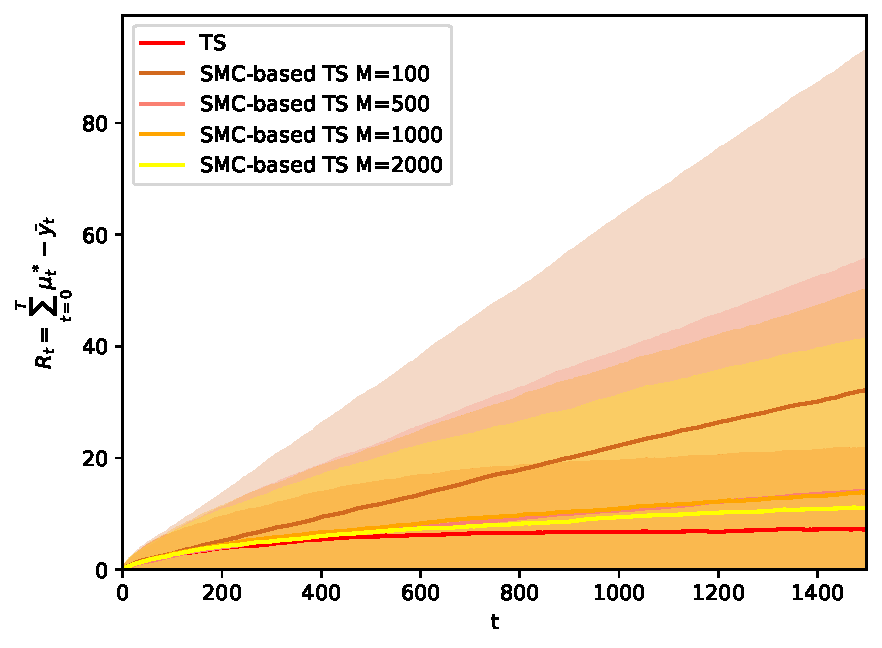
\includegraphics[width=\textwidth]{./fods_figs/static/bernoulli/A2/theta0.8_0.9_allM_cumulative_regret_ts}
		\caption{SMC-based TS: impact of $M$.}
	\end{subfigure}
	\begin{subfigure}[b]{0.46\textwidth}
		\centering
		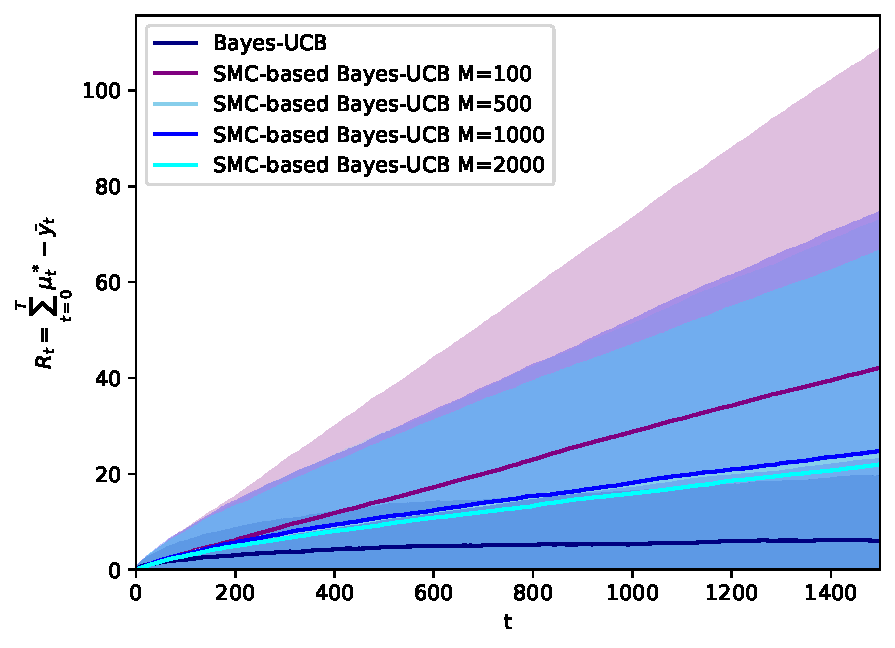
\includegraphics[width=\textwidth]{./fods_figs/static/bernoulli/A2/theta0.8_0.9_allM_cumulative_regret_bucb}
		\caption{SMC-based Bayes-UCB: impact of $M$}
	\end{subfigure}
	
	\caption{Mean cumulative regret (standard deviation shown as the shaded region) of Bayesian policies in a stationary two-armed Bernoulli bandit, with $\theta_0=0.8, \ \theta_1=0.9$.}
\end{figure}

\clearpage
\subsubsection{Bernoulli bandits, A=5}
\label{asssec:static_bandits_bernoulli_5}

We present below cumulative regret results for different parameterizations of 5-armed Bernoulli bandits.

% theta0.1_0.2_0.3_0.4_0.5
\begin{figure}[!h]
	\centering
	\begin{subfigure}[b]{\textwidth}
		\centering
		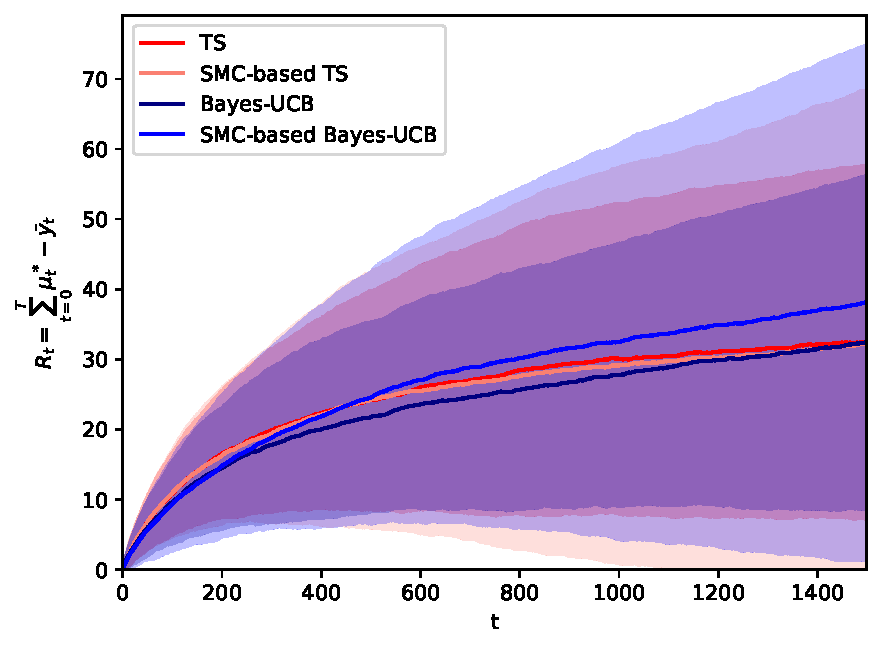
\includegraphics[width=0.75\textwidth]{./fods_figs/static/bernoulli/A5/theta0.1_0.2_0.3_0.4_0.5_M1000_cumulative_regret}
		\caption{Analytical and SMC-based ($M=1000$) TS and Bayes-UCB.}
	\end{subfigure}
	
	\begin{subfigure}[b]{0.46\textwidth}
		\centering
		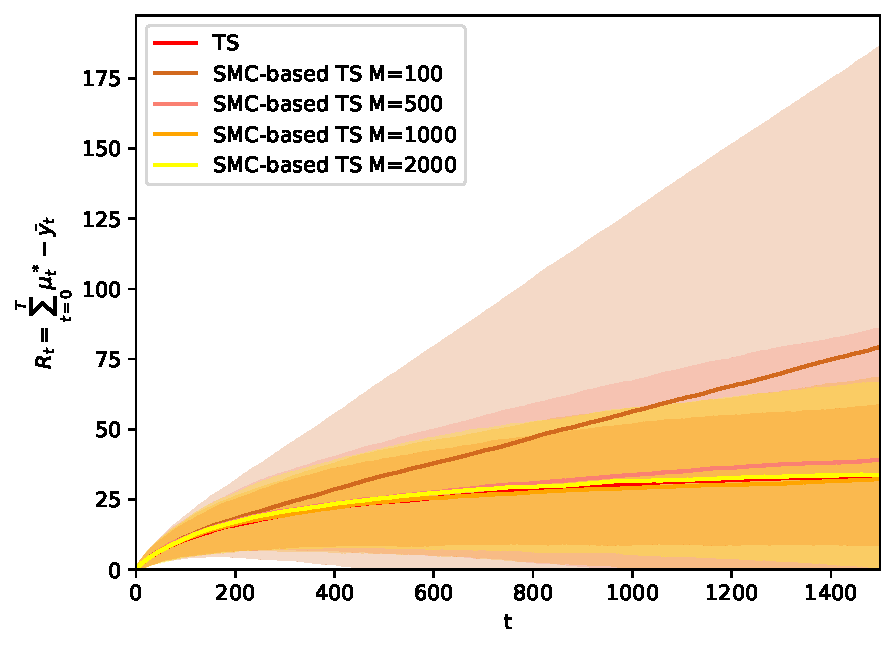
\includegraphics[width=\textwidth]{./fods_figs/static/bernoulli/A5/theta0.1_0.2_0.3_0.4_0.5_allM_cumulative_regret_ts}
		\caption{SMC-based TS: impact of $M$.}
	\end{subfigure}
	\begin{subfigure}[b]{0.46\textwidth}
		\centering
		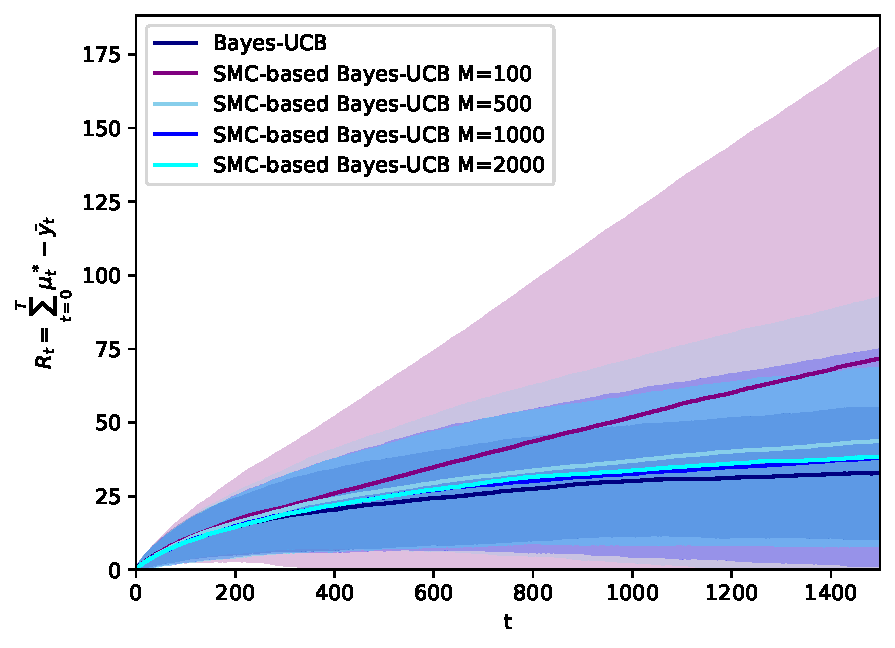
\includegraphics[width=\textwidth]{./fods_figs/static/bernoulli/A5/theta0.1_0.2_0.3_0.4_0.5_allM_cumulative_regret_bucb}
		\caption{SMC-based Bayes-UCB: impact of $M$}
	\end{subfigure}
	
	\caption{Mean cumulative regret (standard deviation shown as the shaded region) of Bayesian policies in a stationary five-armed Bernoulli bandit:
		$\theta_0=0.1, \ \theta_1=0.2, \ \theta_3=0.3, \ \theta_4=0.4, \ \theta_5=0.5$.
	}
\end{figure}

% theta0.1_0.3_0.5_0.6_0.8
\begin{figure}[!h]
	\centering
	\begin{subfigure}[b]{\textwidth}
		\centering
		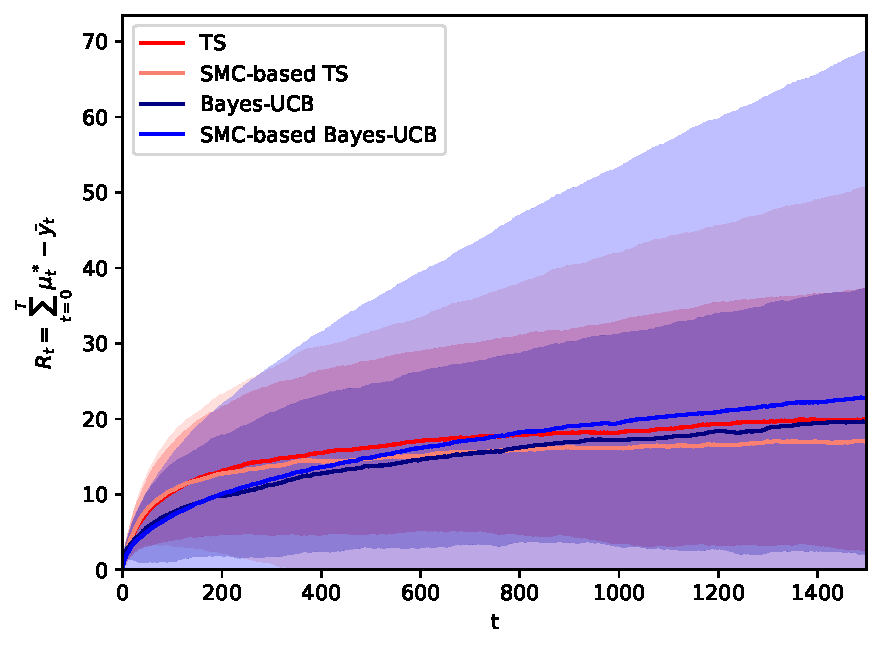
\includegraphics[width=0.75\textwidth]{./fods_figs/static/bernoulli/A5/theta0.1_0.3_0.5_0.6_0.8_M1000_cumulative_regret}
		\caption{Analytical and SMC-based ($M=1000$) TS and Bayes-UCB.}
	\end{subfigure}
	
	\begin{subfigure}[b]{0.46\textwidth}
		\centering
		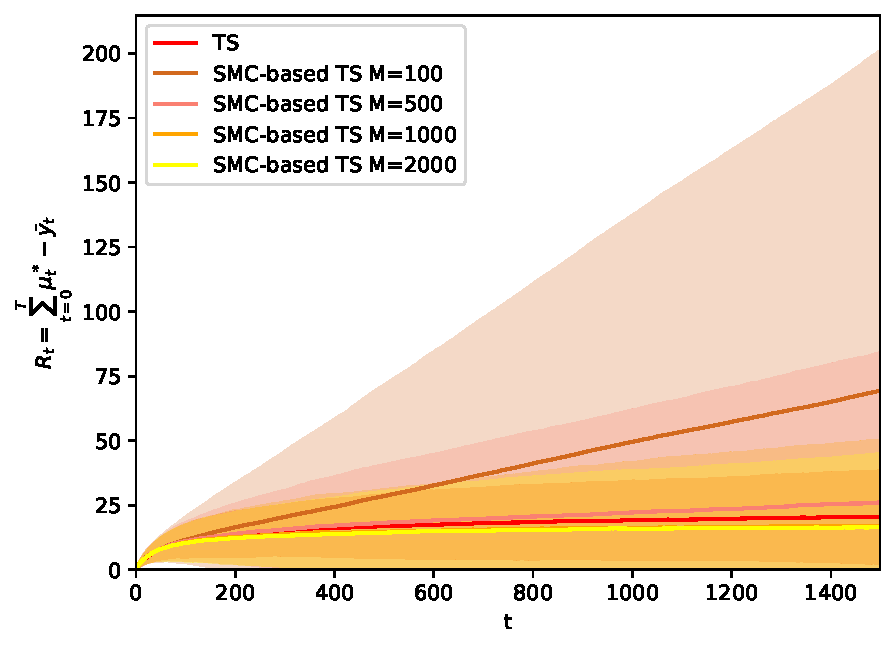
\includegraphics[width=\textwidth]{./fods_figs/static/bernoulli/A5/theta0.1_0.3_0.5_0.6_0.8_allM_cumulative_regret_ts}
		\caption{SMC-based TS: impact of $M$.}
	\end{subfigure}
	\begin{subfigure}[b]{0.46\textwidth}
		\centering
		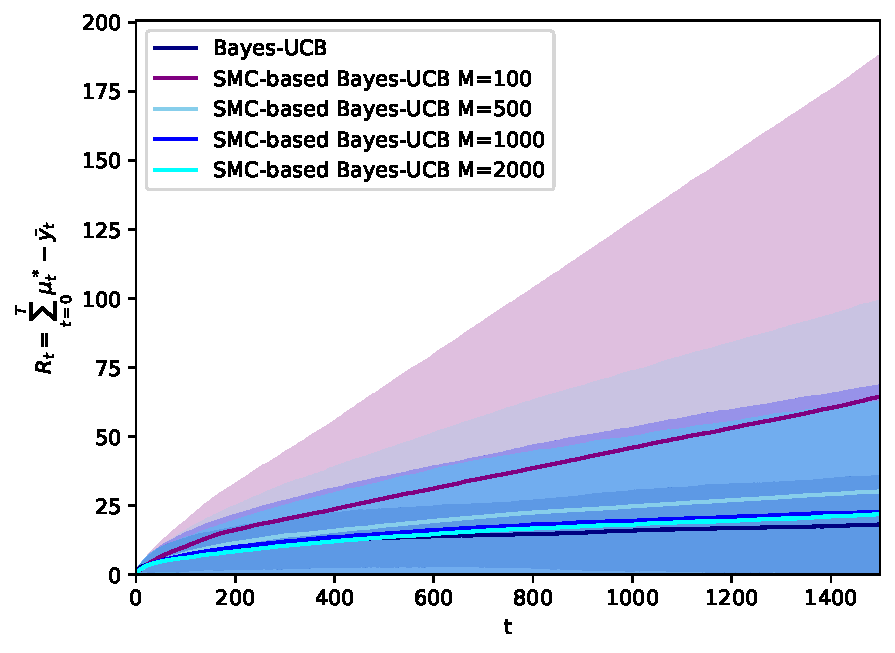
\includegraphics[width=\textwidth]{./fods_figs/static/bernoulli/A5/theta0.1_0.3_0.5_0.6_0.8_allM_cumulative_regret_bucb}
		\caption{SMC-based Bayes-UCB: impact of $M$}
	\end{subfigure}
	
	\caption{Mean cumulative regret (standard deviation shown as the shaded region) of Bayesian policies in a stationary five-armed Bernoulli bandit:
		 $\theta_0=0.1, \ \theta_1=0.3, \ \theta_3=0.5, \ \theta_4=0.6, \ \theta_5=0.8$.
	}
\end{figure}

% theta0.1_0.3_0.5_0.8_0.9
\begin{figure}[!h]
	\centering
	\begin{subfigure}[b]{\textwidth}
		\centering
		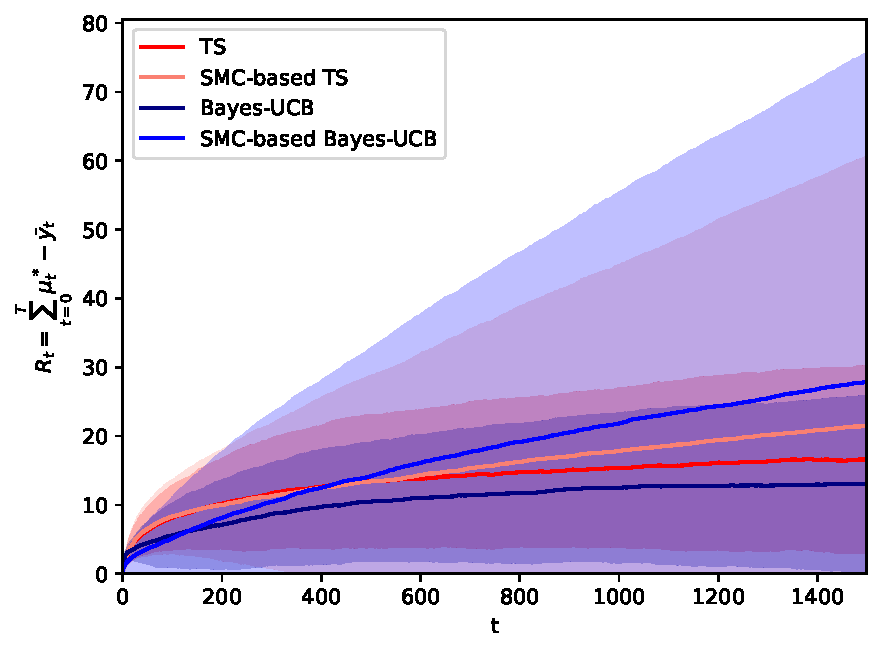
\includegraphics[width=0.75\textwidth]{./fods_figs/static/bernoulli/A5/theta0.1_0.3_0.5_0.8_0.9_M1000_cumulative_regret}
		\caption{Analytical and SMC-based ($M=1000$) TS and Bayes-UCB.}
	\end{subfigure}
	
	\begin{subfigure}[b]{0.46\textwidth}
		\centering
		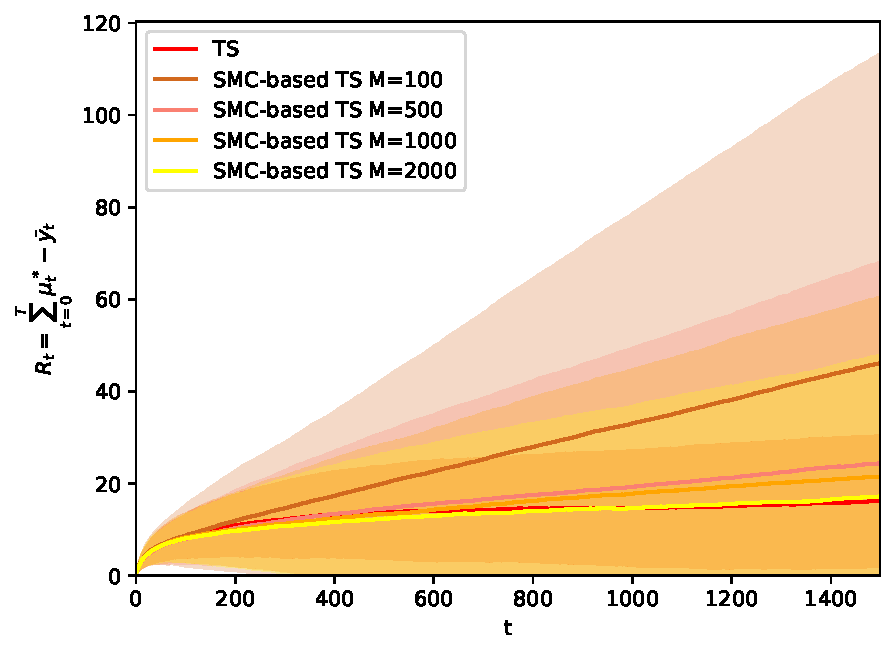
\includegraphics[width=\textwidth]{./fods_figs/static/bernoulli/A5/theta0.1_0.3_0.5_0.8_0.9_allM_cumulative_regret_ts}
		\caption{SMC-based TS: impact of $M$.}
	\end{subfigure}
	\begin{subfigure}[b]{0.46\textwidth}
		\centering
		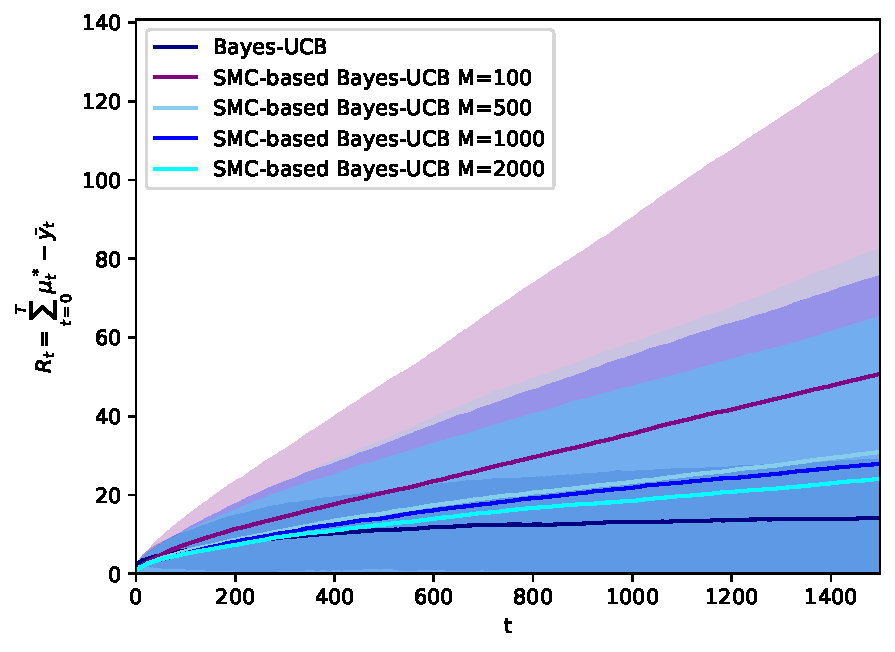
\includegraphics[width=\textwidth]{./fods_figs/static/bernoulli/A5/theta0.1_0.3_0.5_0.8_0.9_allM_cumulative_regret_bucb}
		\caption{SMC-based Bayes-UCB: impact of $M$}
	\end{subfigure}
	
	\caption{Mean cumulative regret (standard deviation shown as the shaded region) of Bayesian policies in a stationary five-armed Bernoulli bandit:
		$\theta_0=0.1, \ \theta_1=0.3, \ \theta_3=0.5, \ \theta_4=0.8, \ \theta_5=0.9$.
	}
\end{figure}

% theta0.1_0.5_0.6_0.7_0.9
\begin{figure}[!h]
	\centering
	\begin{subfigure}[b]{\textwidth}
		\centering
		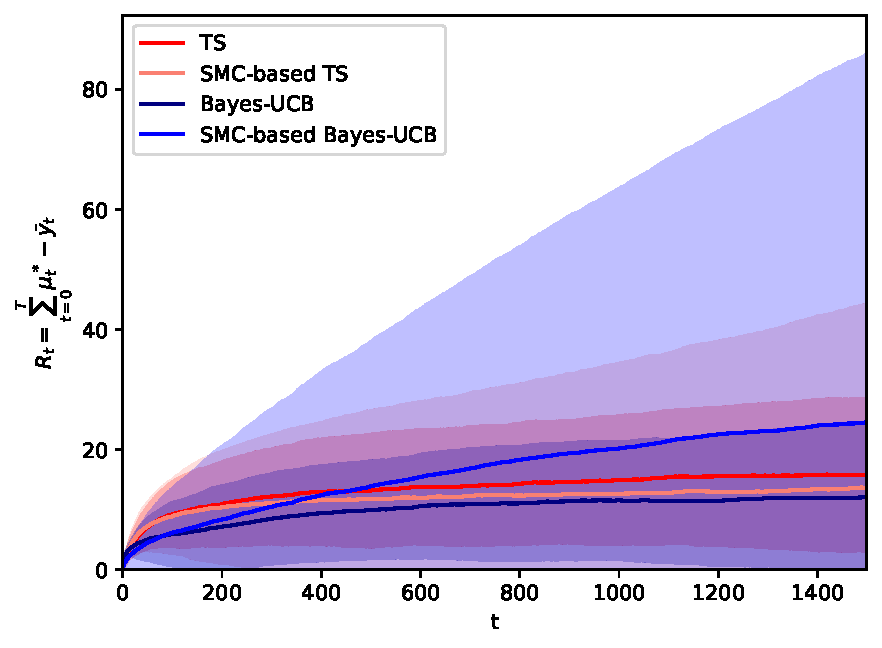
\includegraphics[width=0.75\textwidth]{./fods_figs/static/bernoulli/A5/theta0.1_0.5_0.6_0.7_0.9_M1000_cumulative_regret}
		\caption{Analytical and SMC-based ($M=1000$) TS and Bayes-UCB.}
	\end{subfigure}
	
	\begin{subfigure}[b]{0.46\textwidth}
		\centering
		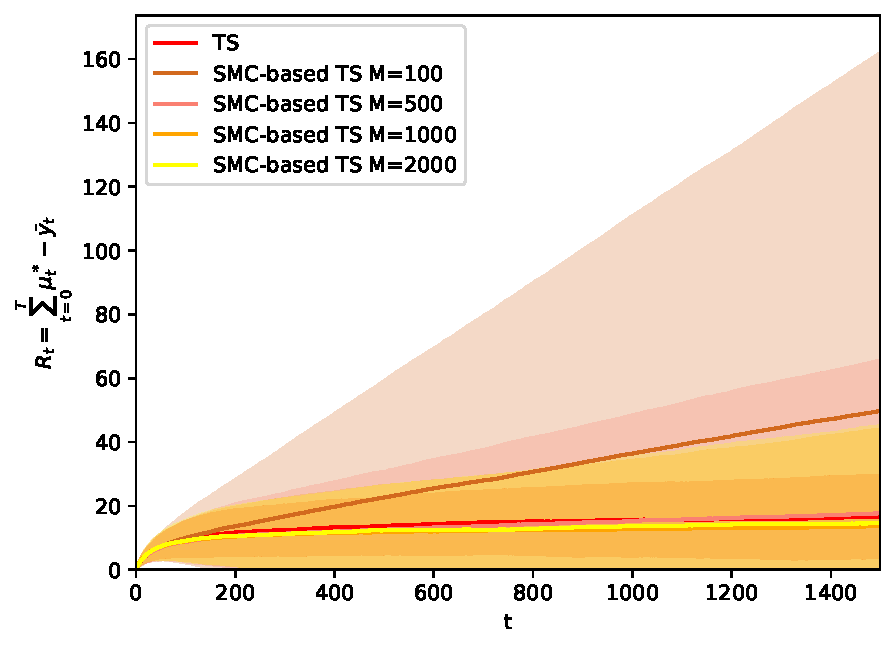
\includegraphics[width=\textwidth]{./fods_figs/static/bernoulli/A5/theta0.1_0.5_0.6_0.7_0.9_allM_cumulative_regret_ts}
		\caption{SMC-based TS: impact of $M$.}
	\end{subfigure}
	\begin{subfigure}[b]{0.46\textwidth}
		\centering
		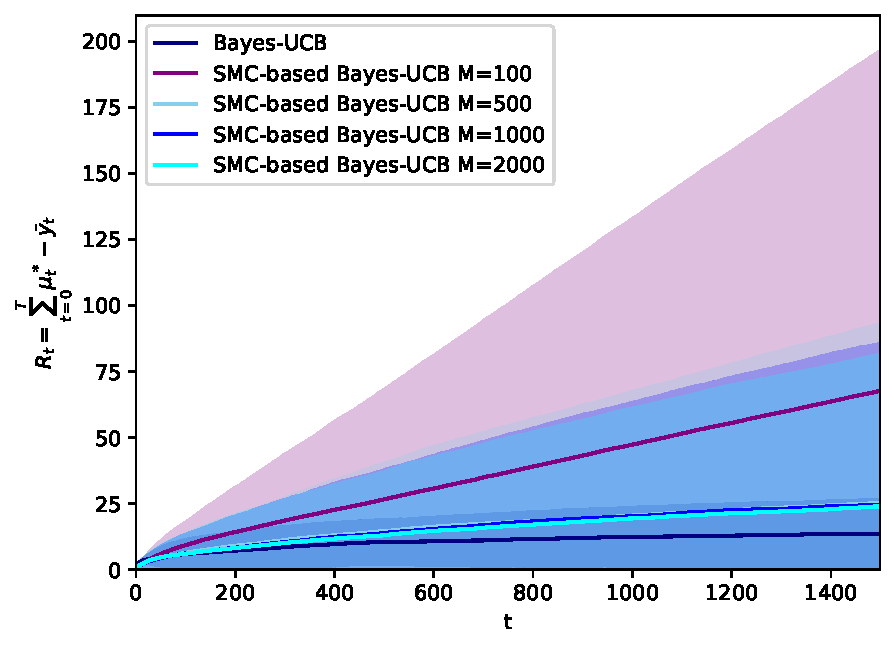
\includegraphics[width=\textwidth]{./fods_figs/static/bernoulli/A5/theta0.1_0.5_0.6_0.7_0.9_allM_cumulative_regret_bucb}
		\caption{SMC-based Bayes-UCB: impact of $M$}
	\end{subfigure}
	
	\caption{Mean cumulative regret (standard deviation shown as the shaded region) of Bayesian policies in a stationary five-armed Bernoulli bandit:
		 $\theta_0=0.1, \ \theta_1=0.5, \ \theta_3=0.6, \ \theta_4=0.7, \ \theta_5=0.9$.
	}
\end{figure}

% theta0.3_0.4_0.5_0.7_0.9
\begin{figure}[!h]
	\centering
	\begin{subfigure}[b]{\textwidth}
		\centering
		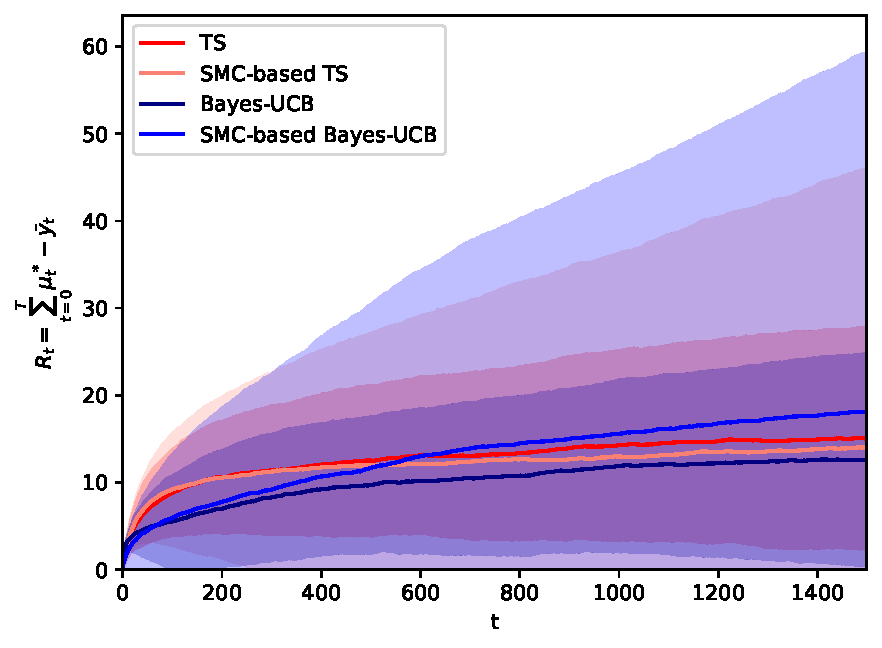
\includegraphics[width=0.75\textwidth]{./fods_figs/static/bernoulli/A5/theta0.3_0.4_0.5_0.7_0.9_M1000_cumulative_regret}
		\caption{Analytical and SMC-based ($M=1000$) TS and Bayes-UCB.}
	\end{subfigure}
	
	\begin{subfigure}[b]{0.46\textwidth}
		\centering
		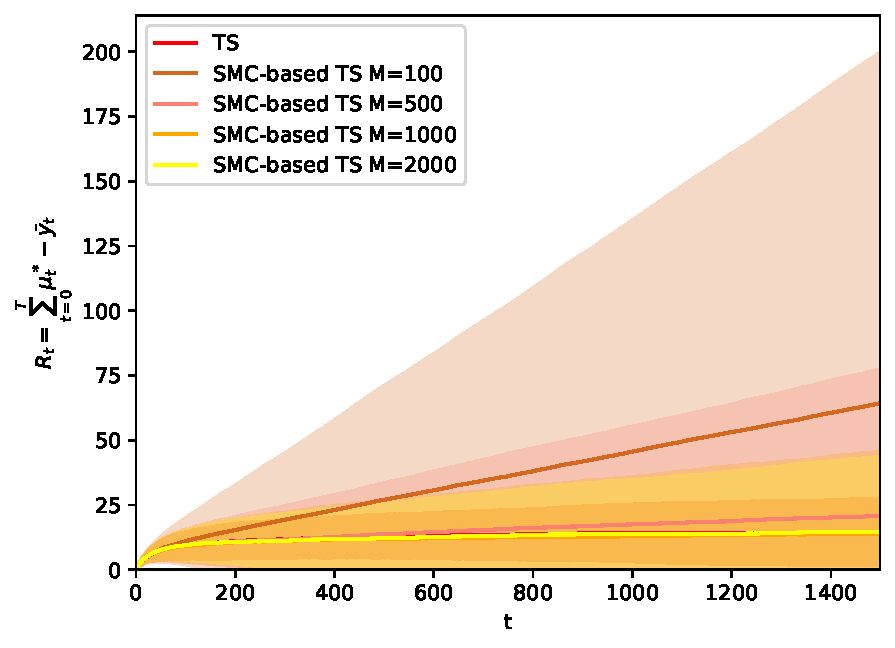
\includegraphics[width=\textwidth]{./fods_figs/static/bernoulli/A5/theta0.3_0.4_0.5_0.7_0.9_allM_cumulative_regret_ts}
		\caption{SMC-based TS: impact of $M$.}
	\end{subfigure}
	\begin{subfigure}[b]{0.46\textwidth}
		\centering
		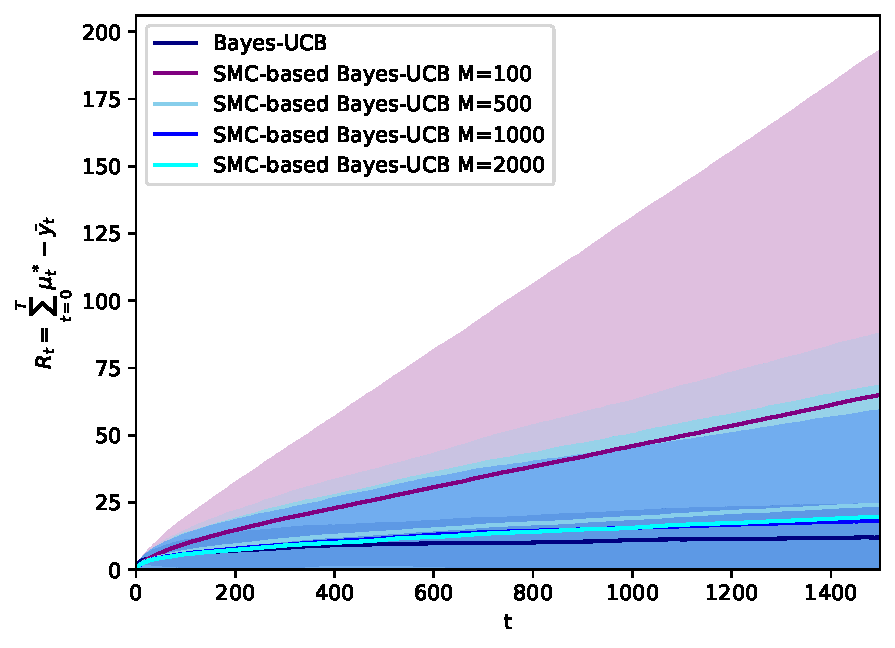
\includegraphics[width=\textwidth]{./fods_figs/static/bernoulli/A5/theta0.3_0.4_0.5_0.7_0.9_allM_cumulative_regret_bucb}
		\caption{SMC-based Bayes-UCB: impact of $M$}
	\end{subfigure}
	
	\caption{Mean cumulative regret (standard deviation shown as the shaded region) of Bayesian policies in a stationary five-armed Bernoulli bandit:
		 $\theta_0=0.3, \ \theta_1=0.4, \ \theta_3=0.5, \ \theta_4=0.7, \ \theta_5=0.9$.
	}
\end{figure}

% theta0.5_0.6_0.7_0.8_0.9
\begin{figure}[!h]
	\centering
	\begin{subfigure}[b]{\textwidth}
		\centering
		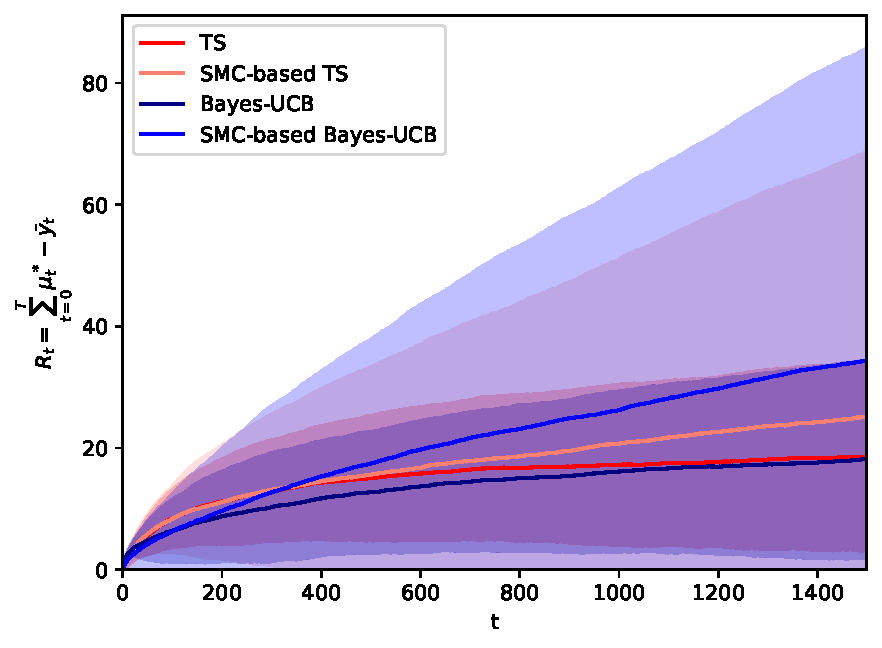
\includegraphics[width=0.75\textwidth]{./fods_figs/static/bernoulli/A5/theta0.5_0.6_0.7_0.8_0.9_M1000_cumulative_regret}
		\caption{Analytical and SMC-based ($M=1000$) TS and Bayes-UCB.}
	\end{subfigure}
	
	\begin{subfigure}[b]{0.46\textwidth}
		\centering
		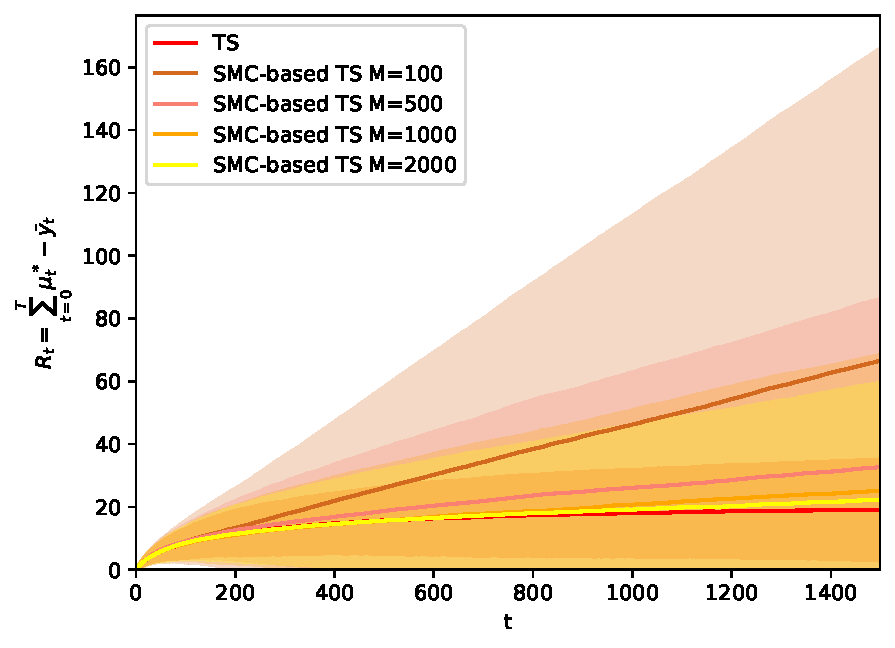
\includegraphics[width=\textwidth]{./fods_figs/static/bernoulli/A5/theta0.5_0.6_0.7_0.8_0.9_allM_cumulative_regret_ts}
		\caption{SMC-based TS: impact of $M$.}
	\end{subfigure}
	\begin{subfigure}[b]{0.46\textwidth}
		\centering
		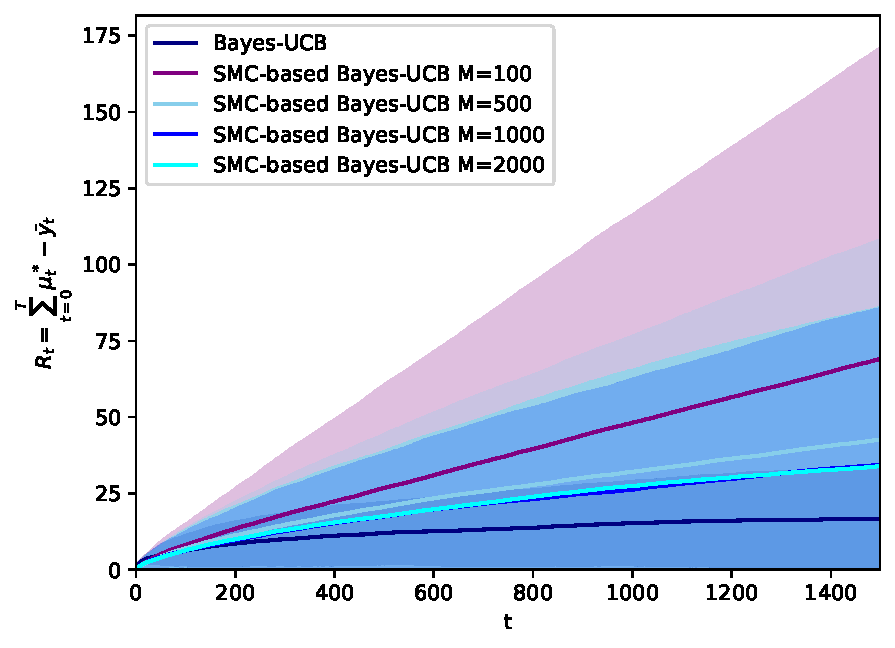
\includegraphics[width=\textwidth]{./fods_figs/static/bernoulli/A5/theta0.5_0.6_0.7_0.8_0.9_allM_cumulative_regret_bucb}
		\caption{SMC-based Bayes-UCB: impact of $M$}
	\end{subfigure}
	
	\caption{Mean cumulative regret (standard deviation shown as the shaded region) of Bayesian policies in a stationary five-armed Bernoulli bandit:
		 $\theta_0=0.5, \ \theta_1=0.6, \ \theta_3=0.7, \ \theta_4=0.8, \ \theta_5=0.9$.
	}
\end{figure}

\clearpage
% !TEX root = smc_bandits.tex

\subsubsection{Contextual Linear Gaussian bandits, A=2}
\label{asssec:static_bandits_linearGaussian_2}

We present below cumulative regret results for different parameterizations of 2-armed, contextual linear Gaussian bandits.

% theta-0.1_-0.1_0.1_0.1_sigma0.5_0.5
\begin{figure}[!h]
	\centering
	\begin{subfigure}[b]{0.46\textwidth}
		\centering
		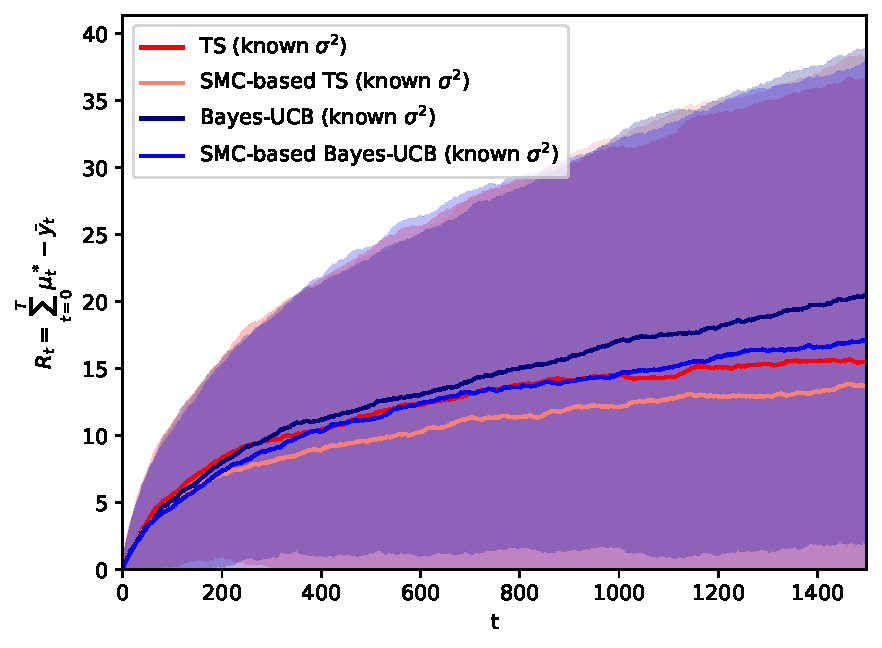
\includegraphics[width=\textwidth]{./fods_figs/static/linear_gaussian/A2/theta-0.1_-0.1_0.1_0.1_sigma0.5_0.5_M1000_cumulative_regret_knownsigma}
		\caption{Known $\sigma$: Analytical and SMC-based ($M=1000$) TS and Bayes-UCB.}
	\end{subfigure}
	\begin{subfigure}[b]{0.46\textwidth}
		\centering
		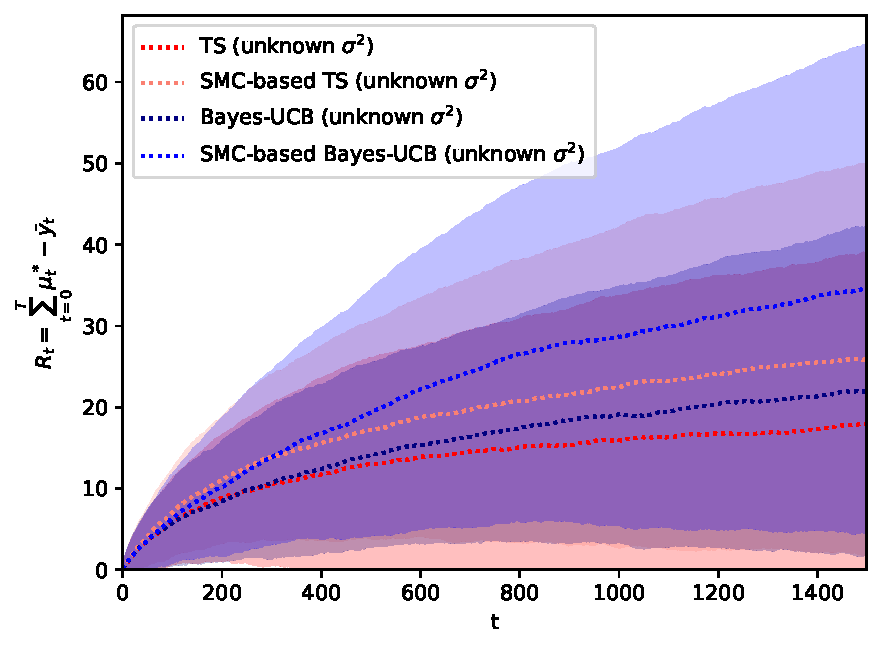
\includegraphics[width=\textwidth]{./fods_figs/static/linear_gaussian/A2/theta-0.1_-0.1_0.1_0.1_sigma0.5_0.5_M1000_cumulative_regret_unknownsigma}
		\caption{Unknown $\sigma$: Analytical and SMC-based ($M=1000$) TS and Bayes-UCB.}
	\end{subfigure}
	
	\begin{subfigure}[b]{0.46\textwidth}
		\centering
		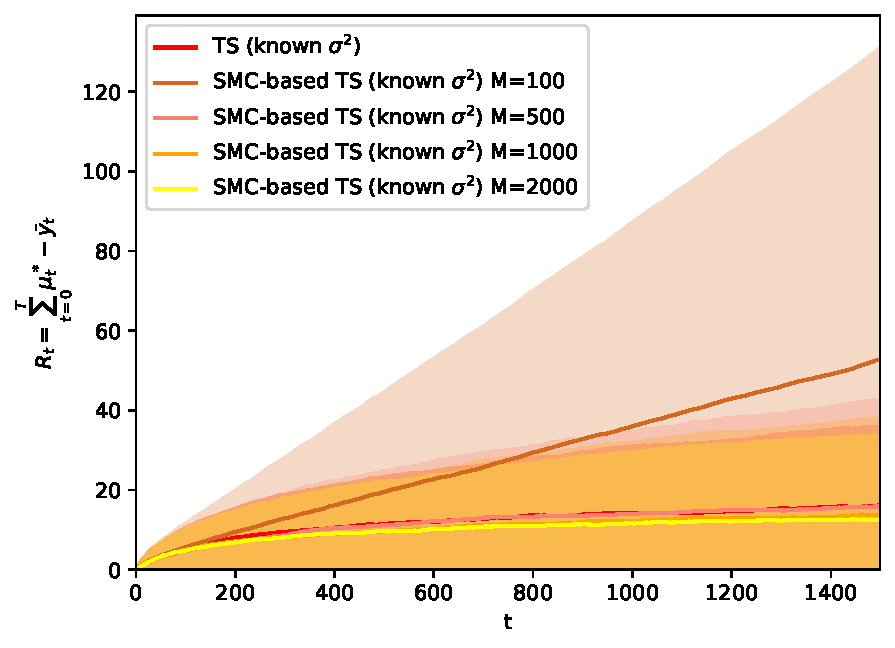
\includegraphics[width=\textwidth]{./fods_figs/static/linear_gaussian/A2/theta-0.1_-0.1_0.1_0.1_sigma0.5_0.5_allM_cumulative_regret_ts_knownsigma}
		\caption{Known $\sigma$: SMC-based TS, \\ impact of $M$.}
	\end{subfigure}
	\begin{subfigure}[b]{0.46\textwidth}
		\centering
		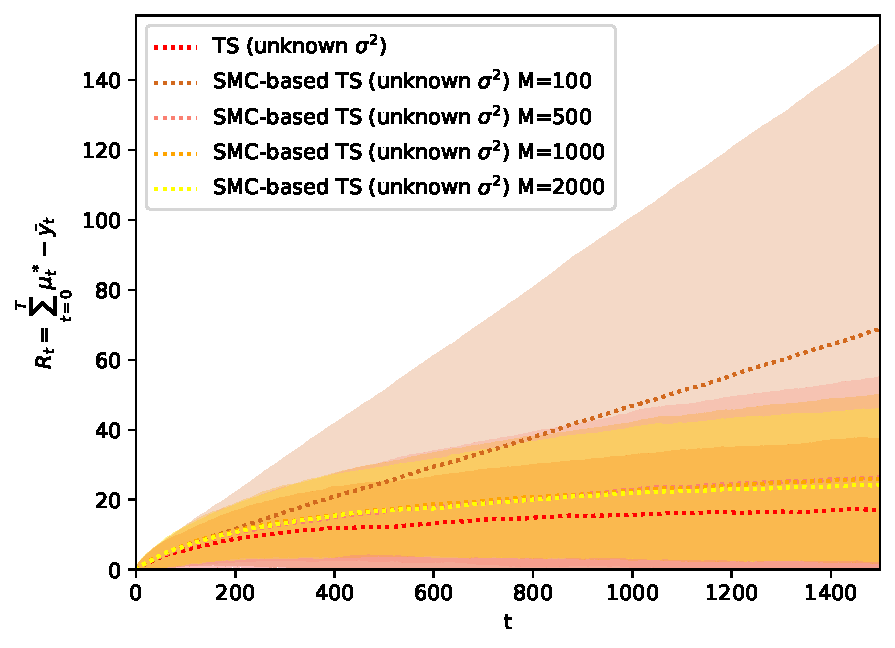
\includegraphics[width=\textwidth]{./fods_figs/static/linear_gaussian/A2/theta-0.1_-0.1_0.1_0.1_sigma0.5_0.5_allM_cumulative_regret_ts_unknownsigma}
		\caption{Unknown $\sigma$: SMC-based TS, \\ impact of $M$.}
	\end{subfigure}

	\begin{subfigure}[b]{0.46\textwidth}
		\centering
		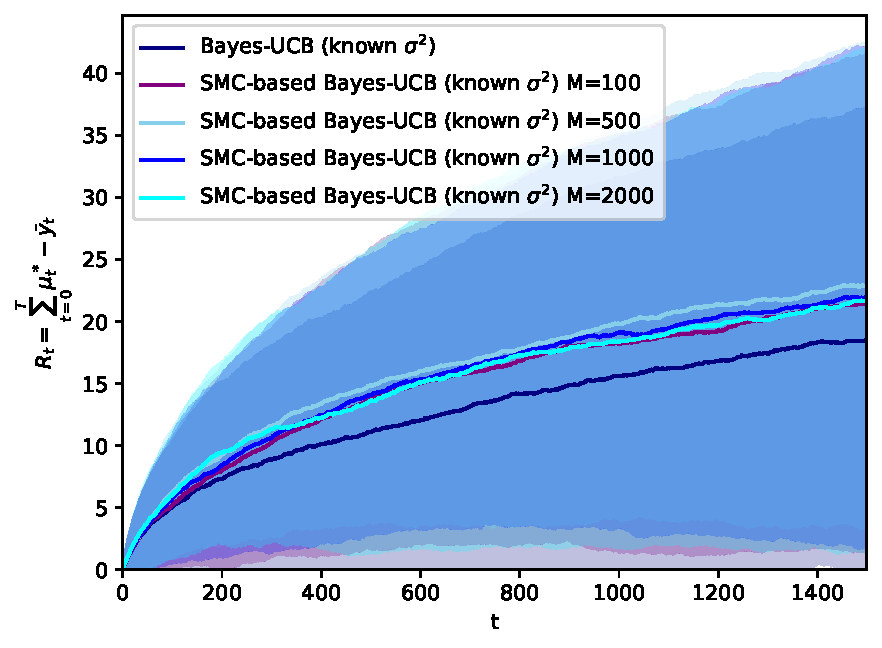
\includegraphics[width=\textwidth]{./fods_figs/static/linear_gaussian/A2/theta-0.1_-0.1_0.1_0.1_sigma0.5_0.5_allM_cumulative_regret_bucb_knownsigma}
		\caption{Known $\sigma$: SMC-based Bayes-UCB, impact of $M$.}
	\end{subfigure}
	\begin{subfigure}[b]{0.46\textwidth}
		\centering
		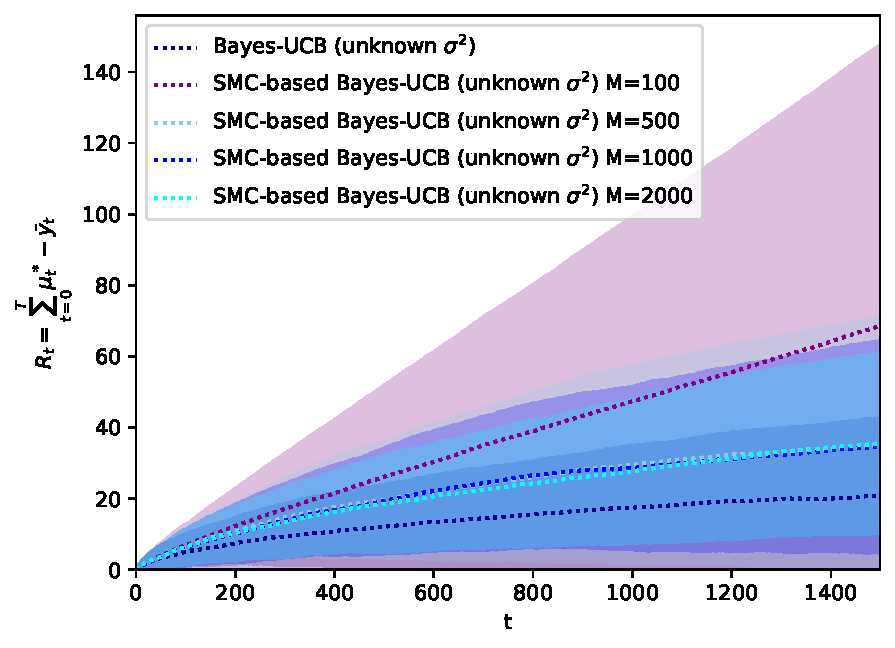
\includegraphics[width=\textwidth]{./fods_figs/static/linear_gaussian/A2/theta-0.1_-0.1_0.1_0.1_sigma0.5_0.5_allM_cumulative_regret_bucb_unknownsigma}
		\caption{Unknown $\sigma$: SMC-based Bayes-UCB, impact of $M$.}
	\end{subfigure}
	
	\caption{Mean cumulative regret (standard deviation shown as the shaded region) of Bayesian policies in a stationary, two-armed contextual Gaussian bandit:
		$\theta_0=(-0.1,-0.1), \ \theta_1=(0.1,0.1), \sigma^2=0.5$.}
\end{figure}

\clearpage
\subsubsection{Contextual Linear Gaussian bandits, A=5}
\label{asssec:static_bandits_linearGaussian_5}

We present below cumulative regret results for different parameterizations of 5-armed, contextual linear Gaussian bandits.

% theta-0.2_-0.2_-0.1_-0.1_0._0._0.1_0.1_0.2_0.2_sigma0.5_0.5_0.5_0.5_0.5
\begin{figure}[!h]
	\centering
	\begin{subfigure}[b]{0.46\textwidth}
		\centering
		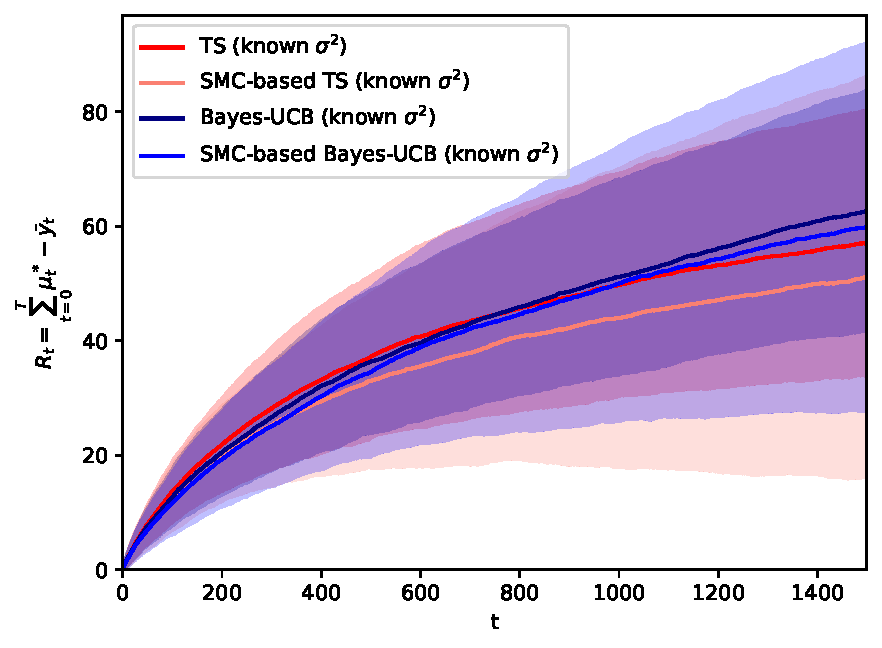
\includegraphics[width=\textwidth]{./fods_figs/static/linear_gaussian/A5/theta-0.2_-0.2_-0.1_-0.1_0._0._0.1_0.1_0.2_0.2_sigma0.5_0.5_0.5_0.5_0.5_M1000_cumulative_regret_knownsigma}
		\caption{Known $\sigma$: Analytical and SMC-based ($M=1000$) TS and Bayes-UCB.}
	\end{subfigure}
	\begin{subfigure}[b]{0.46\textwidth}
		\centering
		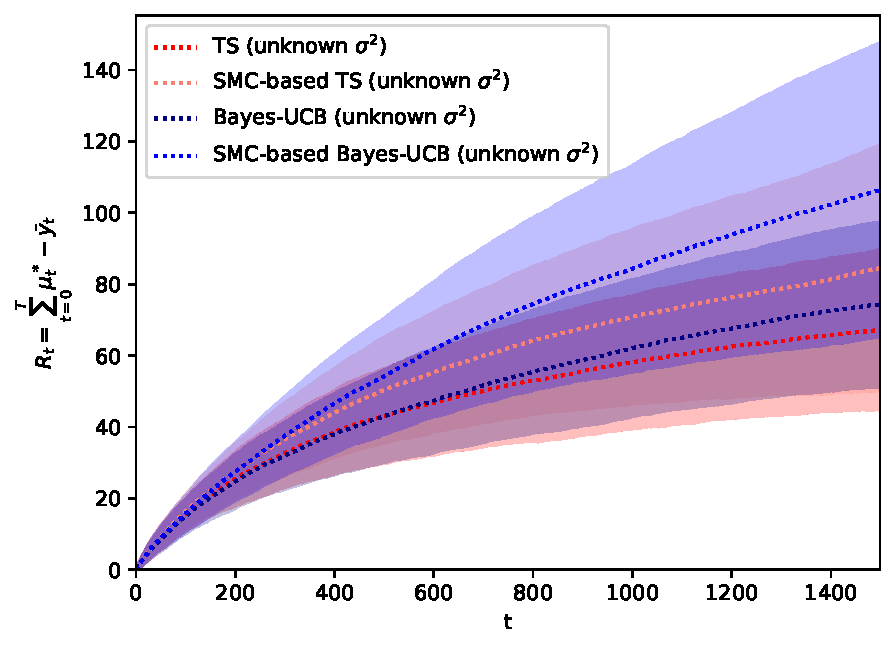
\includegraphics[width=\textwidth]{./fods_figs/static/linear_gaussian/A5/theta-0.2_-0.2_-0.1_-0.1_0._0._0.1_0.1_0.2_0.2_sigma0.5_0.5_0.5_0.5_0.5_M1000_cumulative_regret_unknownsigma}
		\caption{Unknown $\sigma$: Analytical and SMC-based ($M=1000$) TS and Bayes-UCB.}
	\end{subfigure}
	
	\begin{subfigure}[b]{0.46\textwidth}
		\centering
		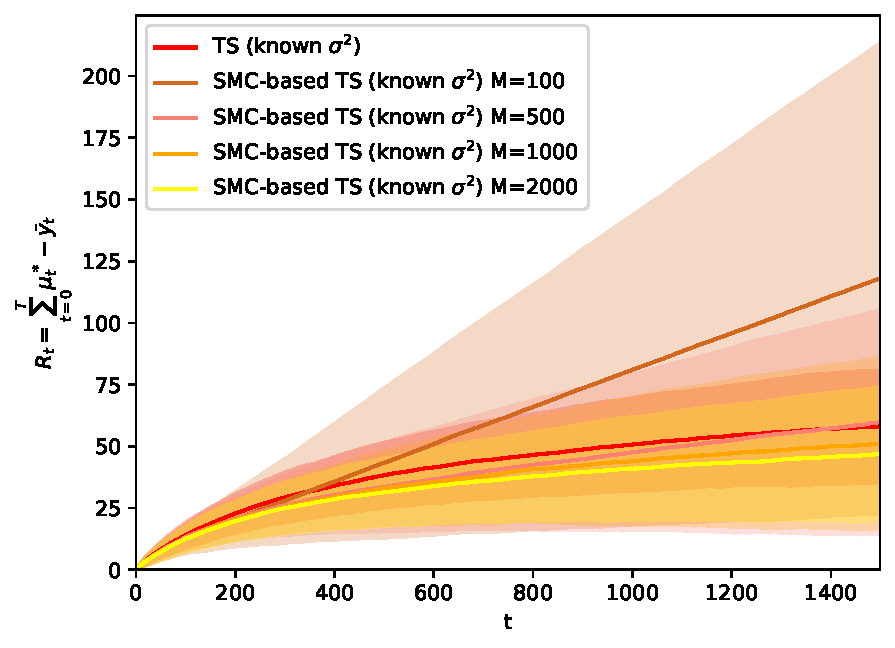
\includegraphics[width=\textwidth]{./fods_figs/static/linear_gaussian/A5/theta-0.2_-0.2_-0.1_-0.1_0._0._0.1_0.1_0.2_0.2_sigma0.5_0.5_0.5_0.5_0.5_allM_cumulative_regret_ts_knownsigma}
		\caption{Known $\sigma$: SMC-based TS, \\ impact of $M$.}
	\end{subfigure}
	\begin{subfigure}[b]{0.46\textwidth}
		\centering
		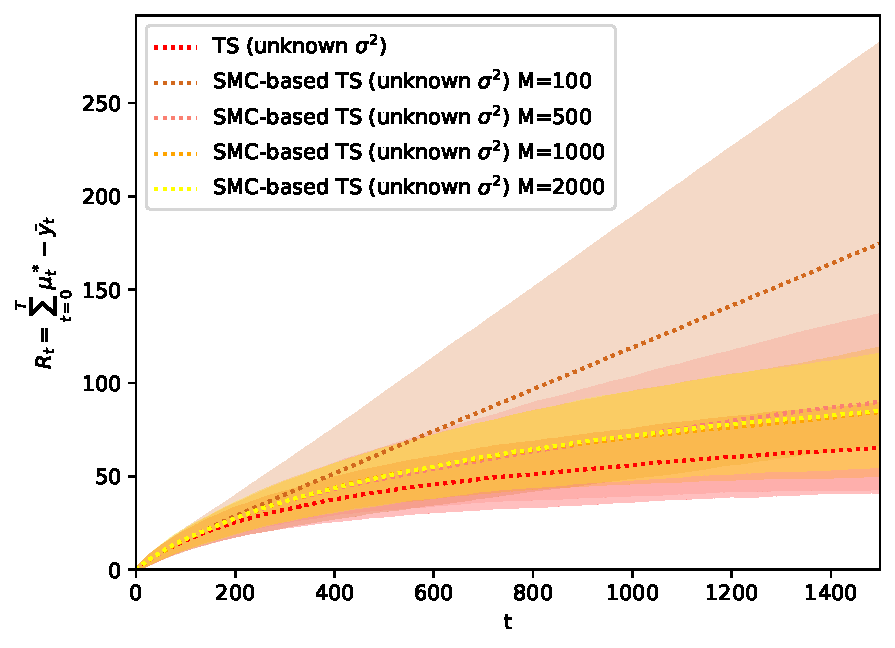
\includegraphics[width=\textwidth]{./fods_figs/static/linear_gaussian/A5/theta-0.2_-0.2_-0.1_-0.1_0._0._0.1_0.1_0.2_0.2_sigma0.5_0.5_0.5_0.5_0.5_allM_cumulative_regret_ts_unknownsigma}
		\caption{Unknown $\sigma$: SMC-based TS, \\ impact of $M$.}
	\end{subfigure}
	
	\begin{subfigure}[b]{0.46\textwidth}
		\centering
		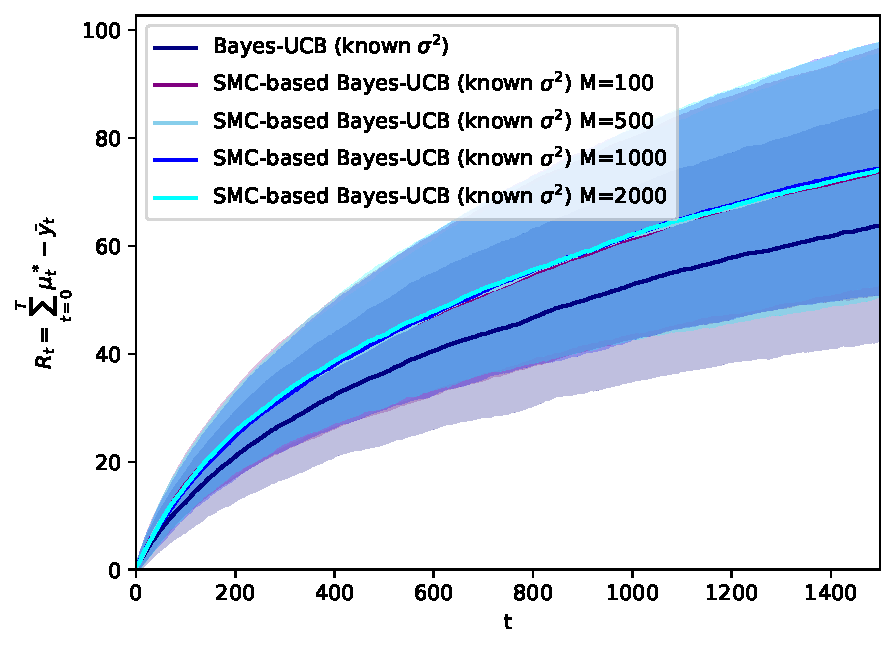
\includegraphics[width=\textwidth]{./fods_figs/static/linear_gaussian/A5/theta-0.2_-0.2_-0.1_-0.1_0._0._0.1_0.1_0.2_0.2_sigma0.5_0.5_0.5_0.5_0.5_allM_cumulative_regret_bucb_knownsigma}
		\caption{Known $\sigma$: SMC-based Bayes-UCB, impact of $M$.}
	\end{subfigure}
	\begin{subfigure}[b]{0.46\textwidth}
		\centering
		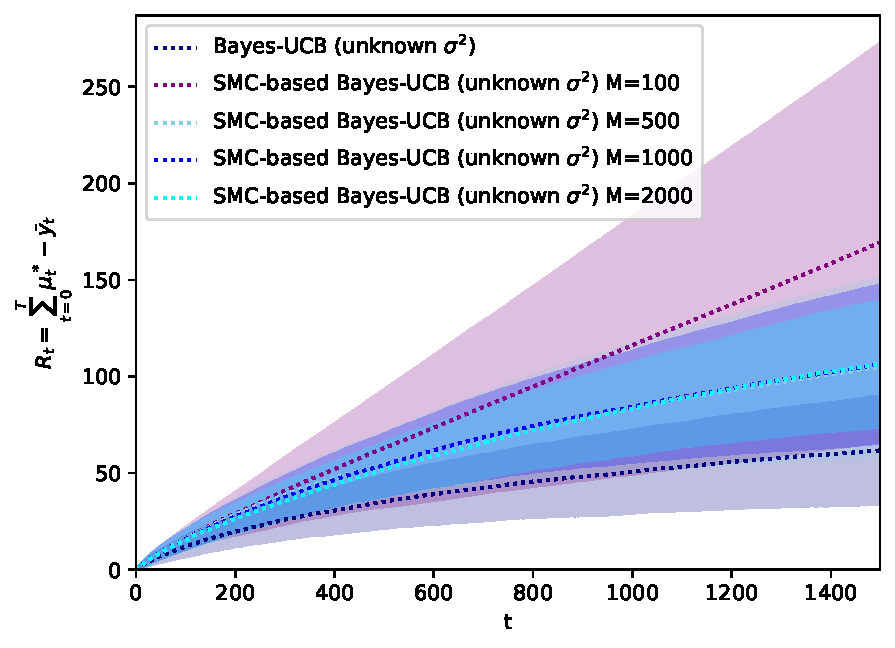
\includegraphics[width=\textwidth]{./fods_figs/static/linear_gaussian/A5/theta-0.2_-0.2_-0.1_-0.1_0._0._0.1_0.1_0.2_0.2_sigma0.5_0.5_0.5_0.5_0.5_allM_cumulative_regret_bucb_unknownsigma}
		\caption{Unknown $\sigma$: SMC-based Bayes-UCB, impact of $M$.}
	\end{subfigure}
	
	\caption{Mean cumulative regret (standard deviation shown as the shaded region) of Bayesian policies in a stationary, five-armed contextual Gaussian bandit: $\theta_0=(-0.2,-0.2), \ \theta_1=(-0.1,-0.1), \ \theta_2=(0,0), \ \theta_3=(0.1,0.1), \ \theta_4=(0.2,0.2), \sigma^2=0.5$.}
\end{figure}

\clearpage
% !TEX root = smc_bandits.tex

\subsection{Experiments with SMC-based Bayesian policies for logistic stationary bandits}
\label{assec:static_bandits_experiments_logistic}

Results in Sections~\ref{asssec:static_bandits_logistic_2} and \ref{asssec:static_bandits_logistic_5}
demonstrate how SMC-based Thompson sampling and Bayes-UCB achieve
successful exploration-exploitation tradeoff, 
for different parameterizations of stationary logistic bandits.
%
This evidence indicates that
the impact of observing context-dependent binary rewards of the played arms is minimal for the proposed SMC-based policies.

The parameter posterior uncertainty associated with SMC-based estimation
is automatically accounted for by both algorithms,
as they explore rarely-played arms if the uncertainty is high.
However, we observe a slight performance deterioration for SMC-based Bayes-UCB,
which we hypothesize is related to the quantile value used ($\alpha_t\propto1/t$).
This decay rate was justified by Kaufmann~\cite{ip-Kaufmann2012} for Bernoulli rewards,
but might not be optimal for other reward functions and,
more importantly, for the SMC-based parameter posterior random measures.

On the contrary, Thompson sampling automatically adjusts
to the uncertainty of the posterior random measure without extra hyperparameter search or tuning,
and attains reduced regret.

\subsubsection{Contextual logistic bandits, A=2}
\label{asssec:static_bandits_logistic_2}

We present below cumulative regret results for different parameterizations of 2-armed, contextual logistic bandits.

% theta-0.1_-0.1_0.1_0.1
\begin{figure}[!h]
	\centering
	\begin{subfigure}[b]{\textwidth}
		\centering
		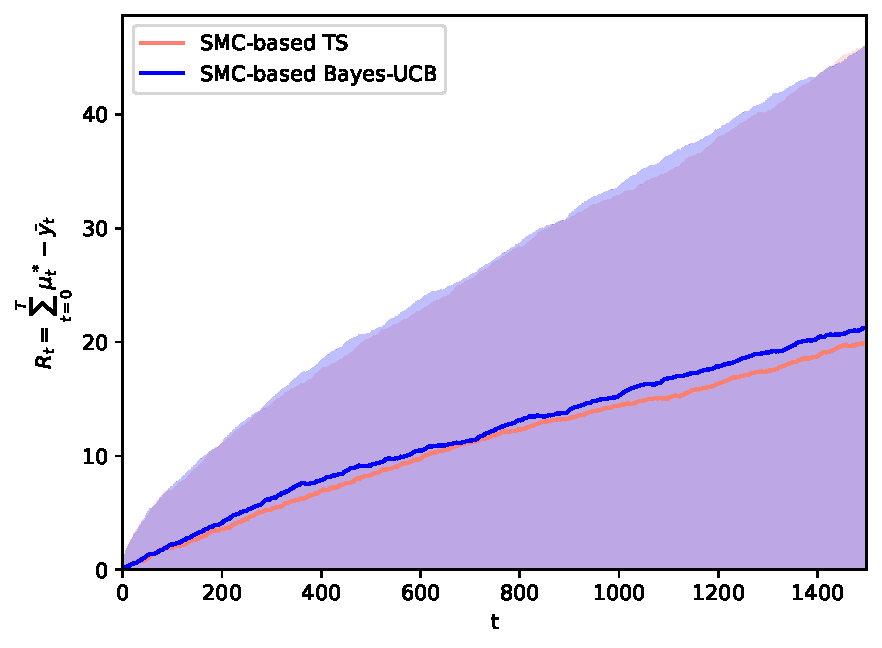
\includegraphics[width=0.75\textwidth]{./fods_figs/static/logistic/A2/theta-0.1_-0.1_0.1_0.1_M1000_cumulative_regret}
		\caption{SMC-based ($M=1000$) TS and Bayes-UCB.}
	\end{subfigure}
	
	\begin{subfigure}[b]{0.46\textwidth}
		\centering
		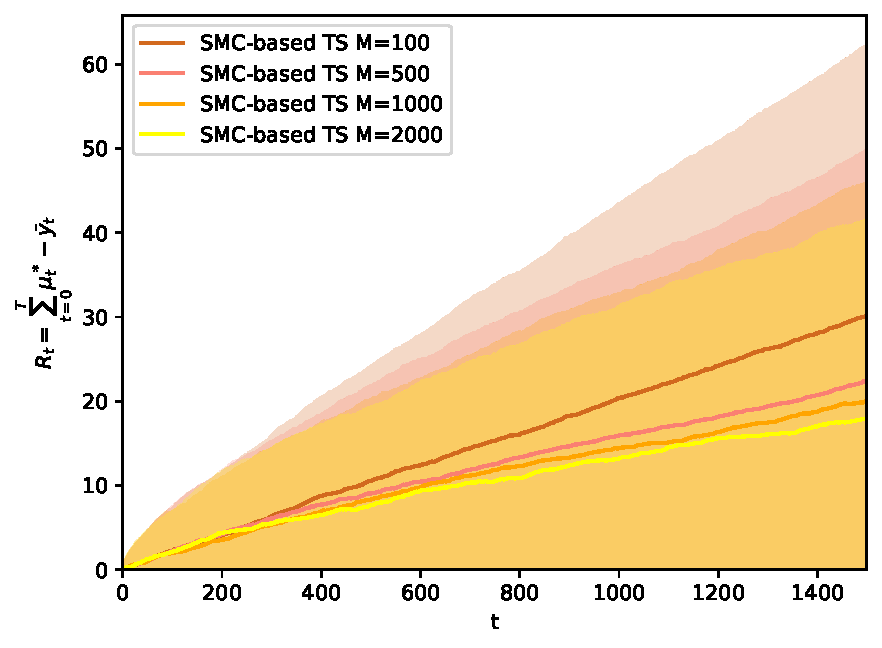
\includegraphics[width=\textwidth]{./fods_figs/static/logistic/A2/theta-0.1_-0.1_0.1_0.1_allM_cumulative_regret_ts}
		\caption{SMC-based TS: impact of $M$.}
	\end{subfigure}
	\begin{subfigure}[b]{0.46\textwidth}
		\centering
		\includegraphics[width=\textwidth]{./fods_figs/static/logistic/A2/theta-0.1_-0.1_0.1_0.1_allM_cumulative_regret_bucb}
		\caption{SMC-based Bayes-UCB: impact of $M$}
	\end{subfigure}
	
	\caption{Mean cumulative regret (standard deviation shown as the shaded region) of SMC-based Bayesian policies in
		stationary, two-armed contextual logistic bandits:
		$\theta_0=(-0.1,-0.1), \ \theta_1=(0.1,0.1)$.}
\end{figure}

% theta-0.5_-0.5_0.5_0.5
\begin{figure}[!h]
	\centering
	\begin{subfigure}[b]{\textwidth}
		\centering
		\includegraphics[width=0.75\textwidth]{./fods_figs/static/logistic/A2/theta-0.5_-0.5_0.5_0.5_M1000_cumulative_regret}
		\caption{SMC-based ($M=1000$) TS and Bayes-UCB.}
	\end{subfigure}
	
	\begin{subfigure}[b]{0.46\textwidth}
		\centering
		\includegraphics[width=\textwidth]{./fods_figs/static/logistic/A2/theta-0.5_-0.5_0.5_0.5_allM_cumulative_regret_ts}
		\caption{SMC-based TS: impact of $M$.}
	\end{subfigure}
	\begin{subfigure}[b]{0.46\textwidth}
		\centering
		\includegraphics[width=\textwidth]{./fods_figs/static/logistic/A2/theta-0.5_-0.5_0.5_0.5_allM_cumulative_regret_bucb}
		\caption{SMC-based Bayes-UCB: impact of $M$}
	\end{subfigure}
	
	\caption{Mean cumulative regret (standard deviation shown as the shaded region) of SMC-based Bayesian policies in
		stationary, two-armed contextual logistic bandits:
		$\theta_0=(-0.5,-0.5), \ \theta_1=(0.5,0.5)$.}
\end{figure}

% theta-1._-1._1._1.
\begin{figure}[!h]
	\centering
	\begin{subfigure}[b]{\textwidth}
		\centering
		\includegraphics[width=0.75\textwidth]{./fods_figs/static/logistic/A2/theta-1._-1._1._1._M1000_cumulative_regret}
		\caption{SMC-based ($M=1000$) TS and Bayes-UCB.}
	\end{subfigure}
	
	\begin{subfigure}[b]{0.46\textwidth}
		\centering
		\includegraphics[width=\textwidth]{./fods_figs/static/logistic/A2/theta-1._-1._1._1._allM_cumulative_regret_ts}
		\caption{SMC-based TS: impact of $M$.}
	\end{subfigure}
	\begin{subfigure}[b]{0.46\textwidth}
		\centering
		\includegraphics[width=\textwidth]{./fods_figs/static/logistic/A2/theta-1._-1._1._1._allM_cumulative_regret_bucb}
		\caption{SMC-based Bayes-UCB: impact of $M$}
	\end{subfigure}
	
	\caption{Mean cumulative regret (standard deviation shown as the shaded region) of SMC-based Bayesian policies in
		stationary, two-armed contextual logistic bandits:
		$\theta_0=(-1.0,-1.0), \ \theta_1=(1.0,1.0)$.}
\end{figure}

\clearpage
\subsubsection{Contextual logistic bandits, A=5}
\label{asssec:static_bandits_logistic_5}

We present below cumulative regret results for different parameterizations of 5-armed, contextual logistic bandits.

% theta-0.2_-0.2_-0.1_-0.1_0._0._0.1_0.1_0.2_0.2
\begin{figure}[!h]
	\centering
	\begin{subfigure}[b]{\textwidth}
		\centering
		\includegraphics[width=0.75\textwidth]{./fods_figs/static/logistic/A5/theta-0.2_-0.2_-0.1_-0.1_0._0._0.1_0.1_0.2_0.2_M1000_cumulative_regret}
		\caption{SMC-based ($M=1000$) TS and Bayes-UCB.}
	\end{subfigure}
	
	\begin{subfigure}[b]{0.46\textwidth}
		\centering
		\includegraphics[width=\textwidth]{./fods_figs/static/logistic/A5/theta-0.2_-0.2_-0.1_-0.1_0._0._0.1_0.1_0.2_0.2_allM_cumulative_regret_ts}
		\caption{SMC-based TS: impact of $M$.}
	\end{subfigure}
	\begin{subfigure}[b]{0.46\textwidth}
		\centering
		\includegraphics[width=\textwidth]{./fods_figs/static/logistic/A5/theta-0.2_-0.2_-0.1_-0.1_0._0._0.1_0.1_0.2_0.2_allM_cumulative_regret_bucb}
		\caption{SMC-based Bayes-UCB: impact of $M$}
	\end{subfigure}
	
	\caption{Mean cumulative regret (standard deviation shown as the shaded region) of SMC-based Bayesian policies in
		stationary, five-armed contextual logistic bandits:
		$\theta_0=(-0.2,-0.2), \ \theta_1=(-0.1,-0.1), \ \theta_2=(0,0), \ \theta_3=(0.1,0.1), \ \theta_4=(0.2,0.2)$.
	}
\end{figure}

% theta-1._-1._-0.5_-0.5_0._0._0.5_0.5_1._1
\begin{figure}[!h]
	\centering
	\begin{subfigure}[b]{\textwidth}
		\centering
		\includegraphics[width=0.75\textwidth]{./fods_figs/static/logistic/A5/theta-1._-1._-0.5_-0.5_0._0._0.5_0.5_1._1._M1000_cumulative_regret}
		\caption{SMC-based ($M=1000$) TS and Bayes-UCB.}
	\end{subfigure}
	
	\begin{subfigure}[b]{0.46\textwidth}
		\centering
		\includegraphics[width=\textwidth]{./fods_figs/static/logistic/A5/theta-1._-1._-0.5_-0.5_0._0._0.5_0.5_1._1._allM_cumulative_regret_ts}
		\caption{SMC-based TS: impact of $M$.}
	\end{subfigure}
	\begin{subfigure}[b]{0.46\textwidth}
		\centering
		\includegraphics[width=\textwidth]{./fods_figs/static/logistic/A5/theta-1._-1._-0.5_-0.5_0._0._0.5_0.5_1._1._allM_cumulative_regret_bucb}
		\caption{SMC-based Bayes-UCB: impact of $M$}
	\end{subfigure}
	
	\caption{Mean cumulative regret (standard deviation shown as the shaded region) of SMC-based Bayesian policies in
		stationary, five-armed contextual logistic bandits:
		$\theta_0=(-1.0,-1.0), \ \theta_1=(-0.5,-0.5), \ \theta_2=(0,0), \ \theta_3=(0.5,0.5), \ \theta_4=(1.0,1.0)$.
	}
\end{figure}

% theta-2._-2._-1._-1._0._0._1._1._2._2.
\begin{figure}[!h]
	\centering
	\begin{subfigure}[b]{\textwidth}
		\centering
		\includegraphics[width=0.75\textwidth]{./fods_figs/static/logistic/A5/theta-2._-2._-1._-1._0._0._1._1._2._2._M1000_cumulative_regret}
		\caption{SMC-based ($M=1000$) TS and Bayes-UCB.}
	\end{subfigure}
	
	\begin{subfigure}[b]{0.46\textwidth}
		\centering
		\includegraphics[width=\textwidth]{./fods_figs/static/logistic/A5/theta-2._-2._-1._-1._0._0._1._1._2._2._allM_cumulative_regret_ts}
		\caption{SMC-based TS: impact of $M$.}
	\end{subfigure}
	\begin{subfigure}[b]{0.46\textwidth}
		\centering
		\includegraphics[width=\textwidth]{./fods_figs/static/logistic/A5/theta-2._-2._-1._-1._0._0._1._1._2._2._allM_cumulative_regret_bucb}
		\caption{SMC-based Bayes-UCB: impact of $M$}
	\end{subfigure}
	
	\caption{Mean cumulative regret (standard deviation shown as the shaded region) of SMC-based Bayesian policies in
		stationary, five-armed contextual logistic bandits:
		$\theta_0=(-2.0,-2.0), \ \theta_1=(-1.0,-1.0), \ \theta_2=(0,0), \ \theta_3=(1.0,1.0), \ \theta_4=(2.0,2.0)$.
	}
\end{figure}
